\chapter{Διερεύνηση Χρονοσειράς \tl{B}}
\label{ch:step3}
\thispagestyle{fancy}

Στις ενότητες και υπο-ενότητες που ακολουθούν γίνεται η ανάλυση της δεύτερης χρονοσειράς ή της \textquote{\tl{B}}. Ακολουθείται ίδια λογική με αυτή της \textquote{\tl{A}}, δηλαδή αρχικά παρατίθενται στοιχεία της αρχικής χρονοσειράς των προβολών, κατόπιν γίνεται σταθεροποίηση διασποράς και απαλοιφή στοχαστικής τάσης. Ώστοσο, όπως αναλύεται παρακάτω, η συγκεκριμένη χρονοσειρά φαίνεται να έχει κάποια εποχικότητα η οποία εκτιμάται και απαλείφεται. Τέλος, προσαρμόζονται $ARMA$ μοντέλα στην απαλλαγμένη από εποχικότητα στάσιμη χρονοσειρά και διεξάγονται οι αντίστοιχες διαγνώσεις καταλληλότητας των γραμμικών μοντέλων.

\section{Αρχική Ανάλυση}

Αρχικά, δίνεται το διάγραμμα ιστορίας της χρονοσειράς \tl{B}, $\{Y_b(t)\}$, ακολούθως.

\begin{figure}[H]
    \begin{center}
        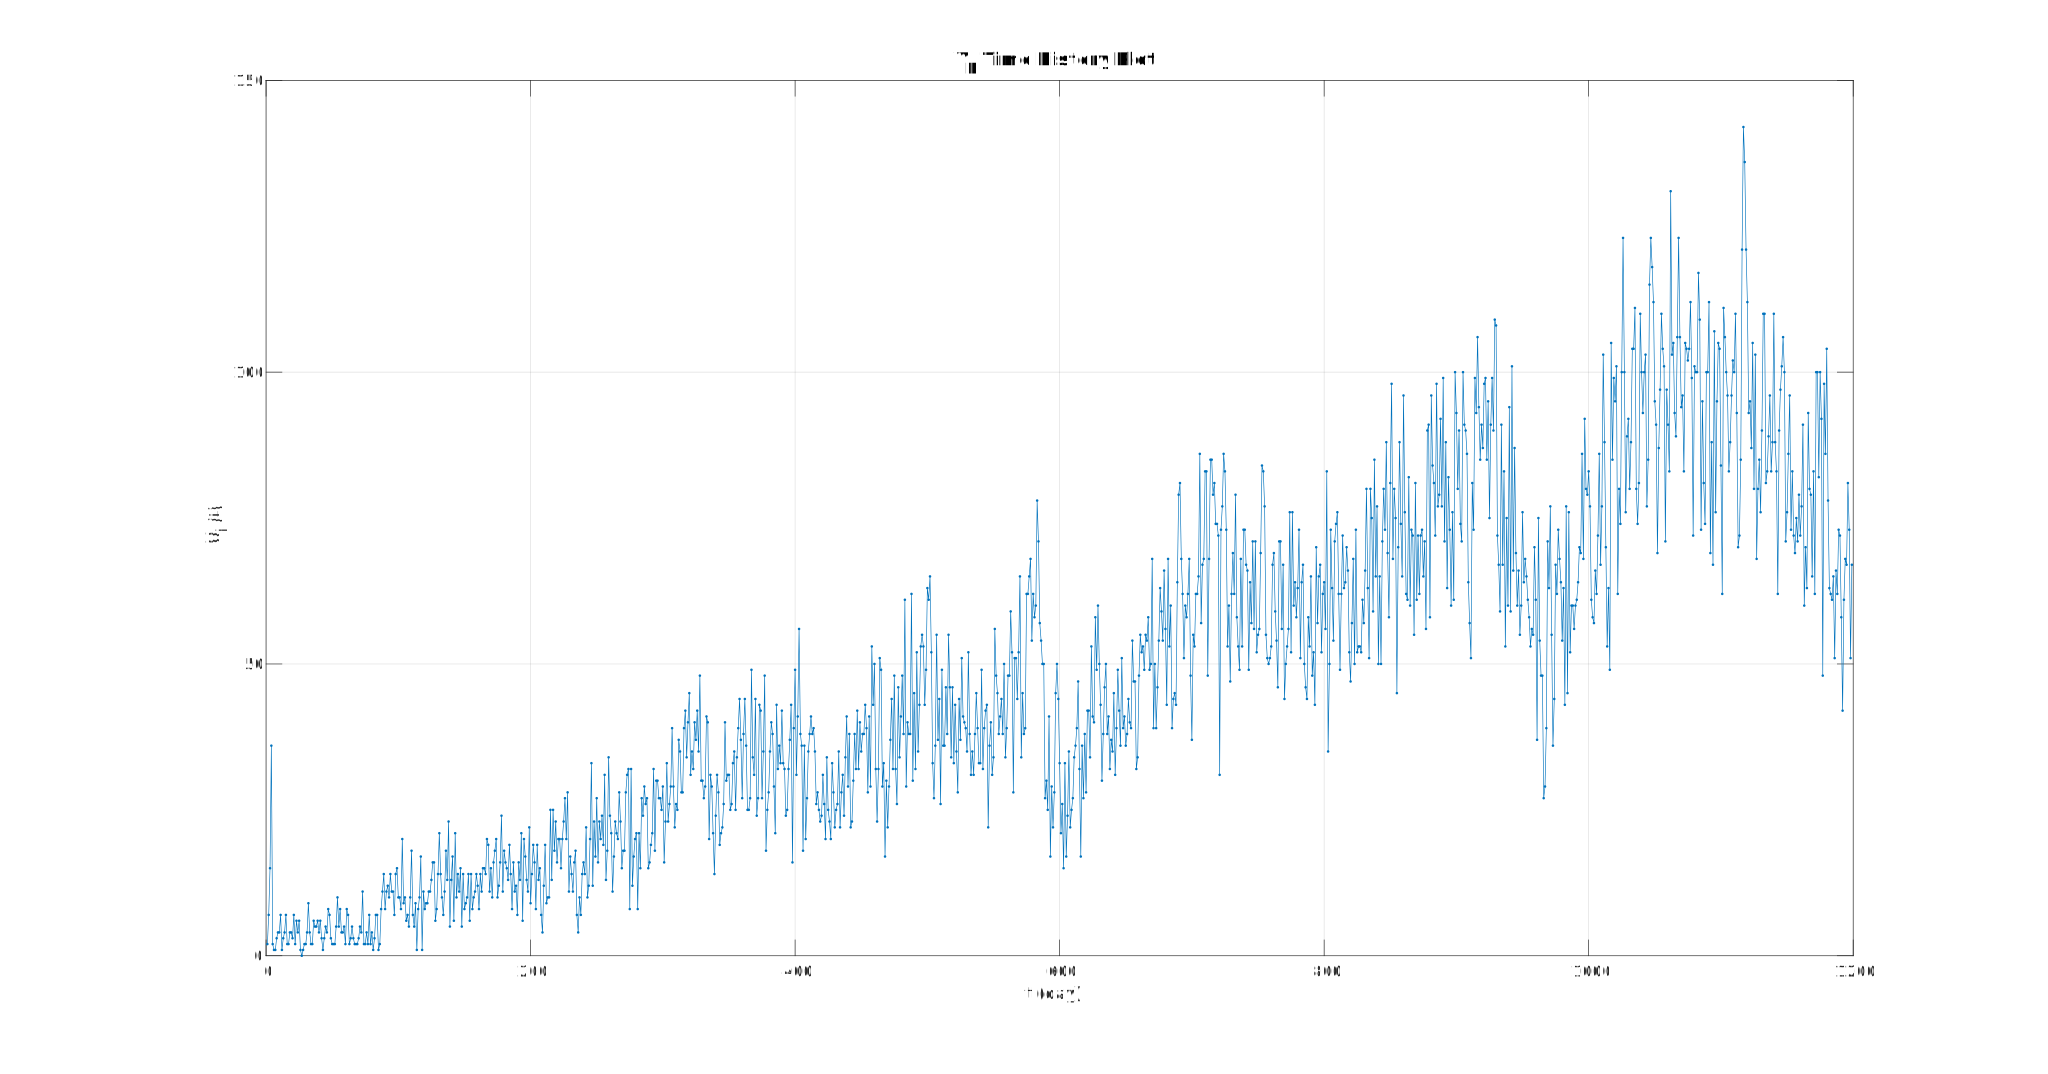
\includegraphics[width=\textwidth]{plots/yb_history.svg.pdf}
        \caption{Διάγραμμα ιστορίας της χρονοσειράς \tl{B}, $\{Y_b(t)\}$, μαζί με τη καμπύλη \tl{MA(7) smoothing}}
        \label{fig:yb_history}
    \end{center}
\end{figure}

Από το διάγραμμα ιστορίας της $\{Y_b(t)\}$ φαίνεται πως η χρονοσειρά δεν είναι στάσιμη καθώς παρατηρείται έντονη αυξητική τάση. Αυτό επιβεβαιώνεται και από τα διαγράμματα της (δειγματικής) αυτοσυσχέτισης και (δειγματικής) μερικής αυτοσυσχέτισης που παρατίθενται ακολούθως:

\begin{figure}[H]
    \begin{center}
        \includegraphics[width=\textwidth]{plots/yb_autocorrelation.svg.pdf}
        \caption{Διάγραμμα (δειγματικής) αυτοσυσχέτισης της χρονοσειράς \tl{B}, $r_y(\tau)$, μαζί με τα όρια σημαντικότητας για 95\% επίπεδο εμπιστοσύνης}
        \label{fig:yb_autocorrelation}
    \end{center}
\end{figure}

\begin{figure}[H]
    \begin{center}
        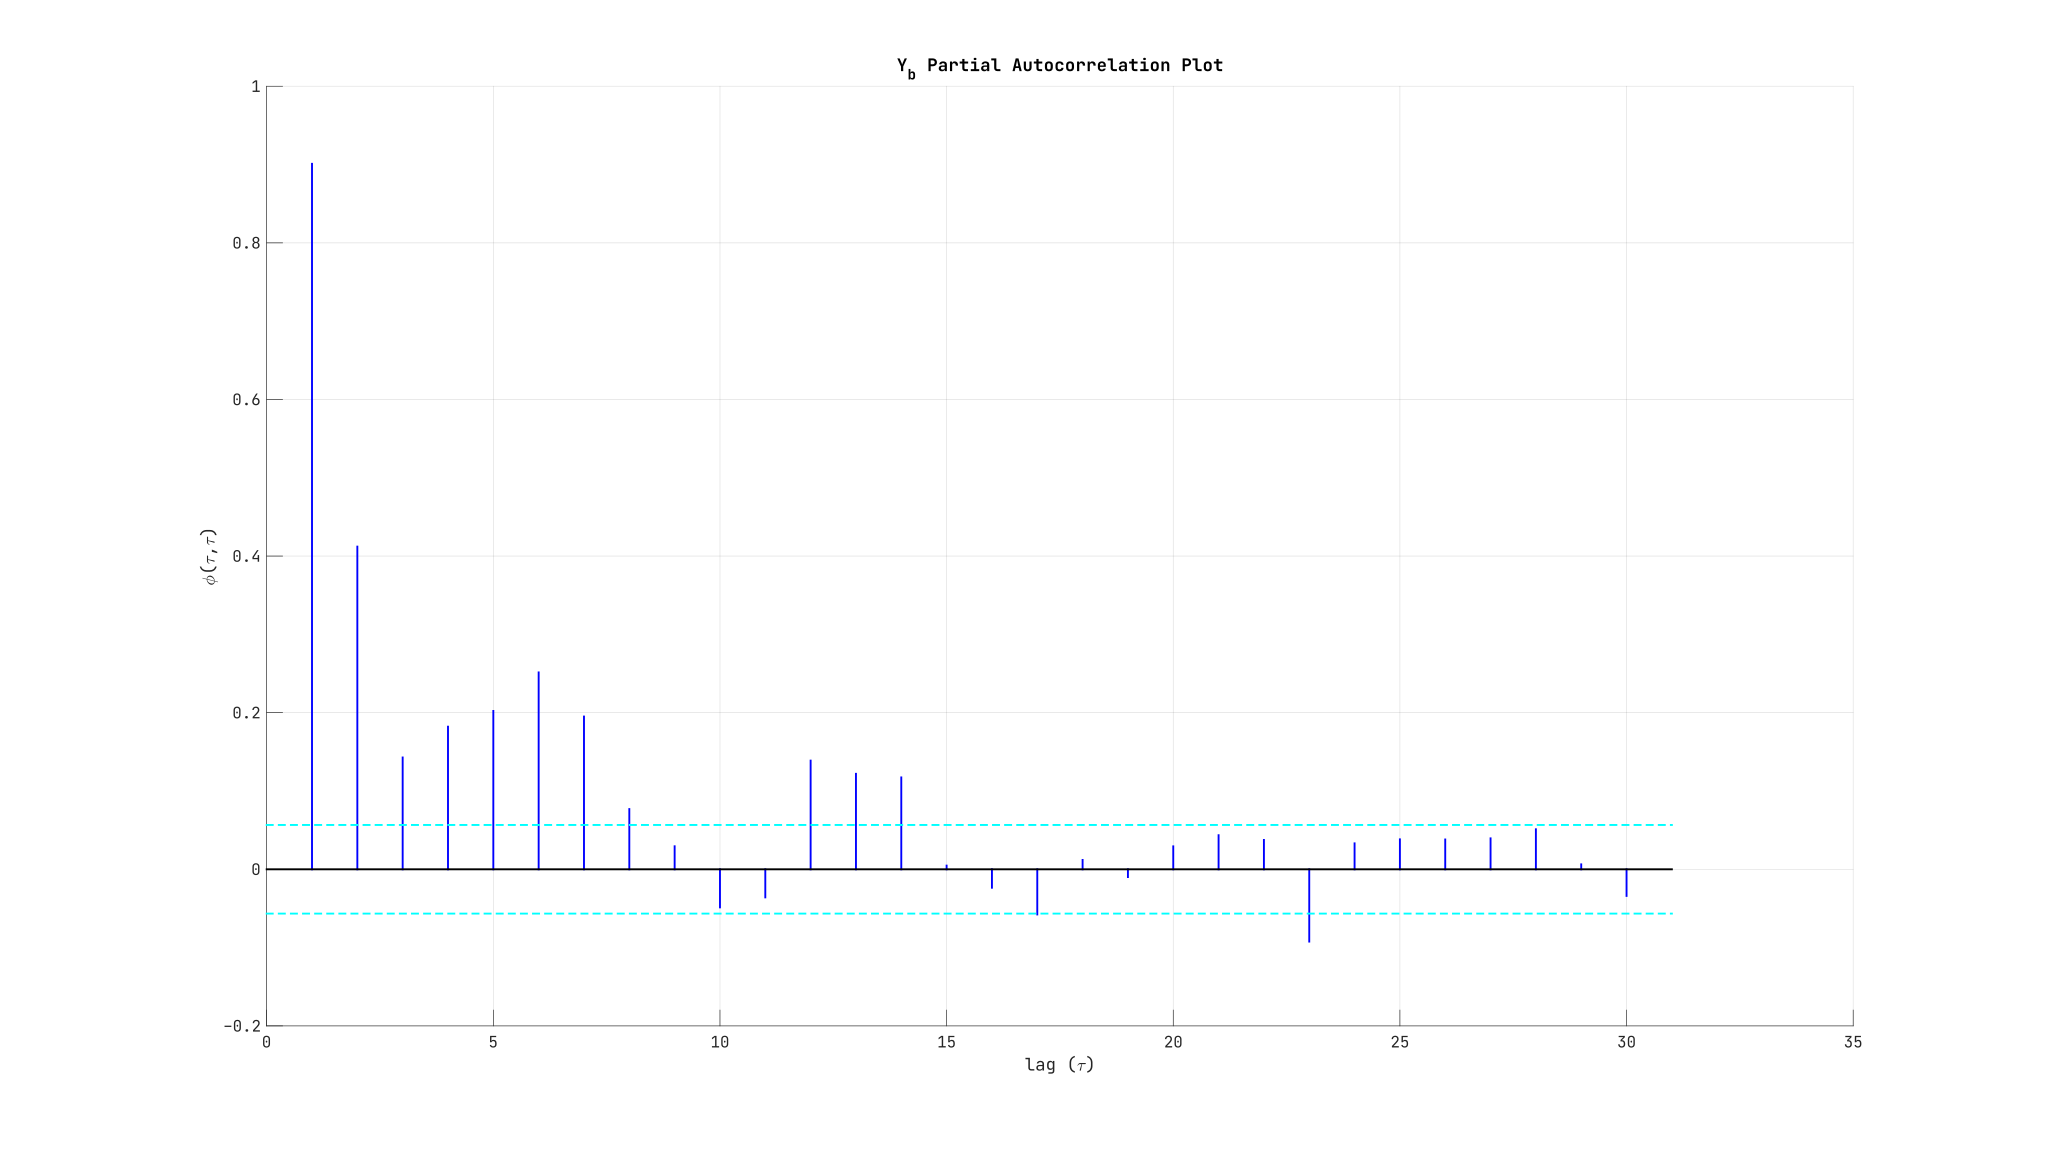
\includegraphics[width=\textwidth]{plots/yb_partial_autocorrelation.svg.pdf}
        \caption{Διάγραμμα (δειγματικής) μερικής αυτοσυσχέτισης της χρονοσειράς \tl{B}, $\phi_y(\tau)$, μαζί με τα όρια σημαντικότητας για 95\% επίπεδο εμπιστοσύνης}
        \label{fig:yb_partial_autocorrelation}
    \end{center}
\end{figure}

Στα παραπάνω διαγράμματα έχουν σημειωθεί και τα όρια σημαντικότητας για επίπεδο εμπιστοσύνης 95\%. Ειδικά στο διάγραμμα αυτοσυσχέτισης φαίνεται έντονα η ύπαρξη τάσης καθώς η αυτοσυσχέτιση έχει υψηλές τιμές και φθίνει πολύ αργά. Η τάση, όπως φαίνεται από το διάγραμμα ιστορίας (σχήμα \ref{fig:yb_history}), είναι στοχαστική και επομένως για να γίνει στάσιμη η χρονοσειρά θα πρέπει να εφαρμοστεί κάποια μέθοδος απαλοιφής της στοχαστικής τάσης (όπως η μέθοδος των πρώτων διαφορών). Επίσης, αμυδρά φαίνεται στο διάγραμμα αυτοσυσχέτισης και ύπαρξη κάποιας περιοδίκοτητας, όμως αυτή θα φανεί πιο καθαρά παρακάτω.

\section{Απαλοιφή Στοχαστικής Τάσης}

Για την απαλοιφή της τάσης αρχικά δοκιμάστηκαν οι πρώτες διαφορές. Η χρονοσειρά που προκύπτει λοιπόν θα είναι:
\begin{align}
    BY_b(t) = Y_b(t) - Y_b(t-1)
\end{align}

Παρακάτω παρατίθεται το διάγραμμα ιστορίας της $\{BY_b(t)\}$ όπου φαίνεται ότι ο μετασχηματισμός των πρώτων διαφορών έχει καταφέρει να απαλείψει τη στοαχαστική τάση και επομένως δεν υπάρχει η ανάγκη για επανάληψη της διαδικασίας (δηλαδή να πάρω διαφορές δεύτερης τάξης) ή για προσφυγή σε άλλη μέθοδο απαλοιφής στοχαστικής τάσης.

\begin{figure}[H]
    \begin{center}
        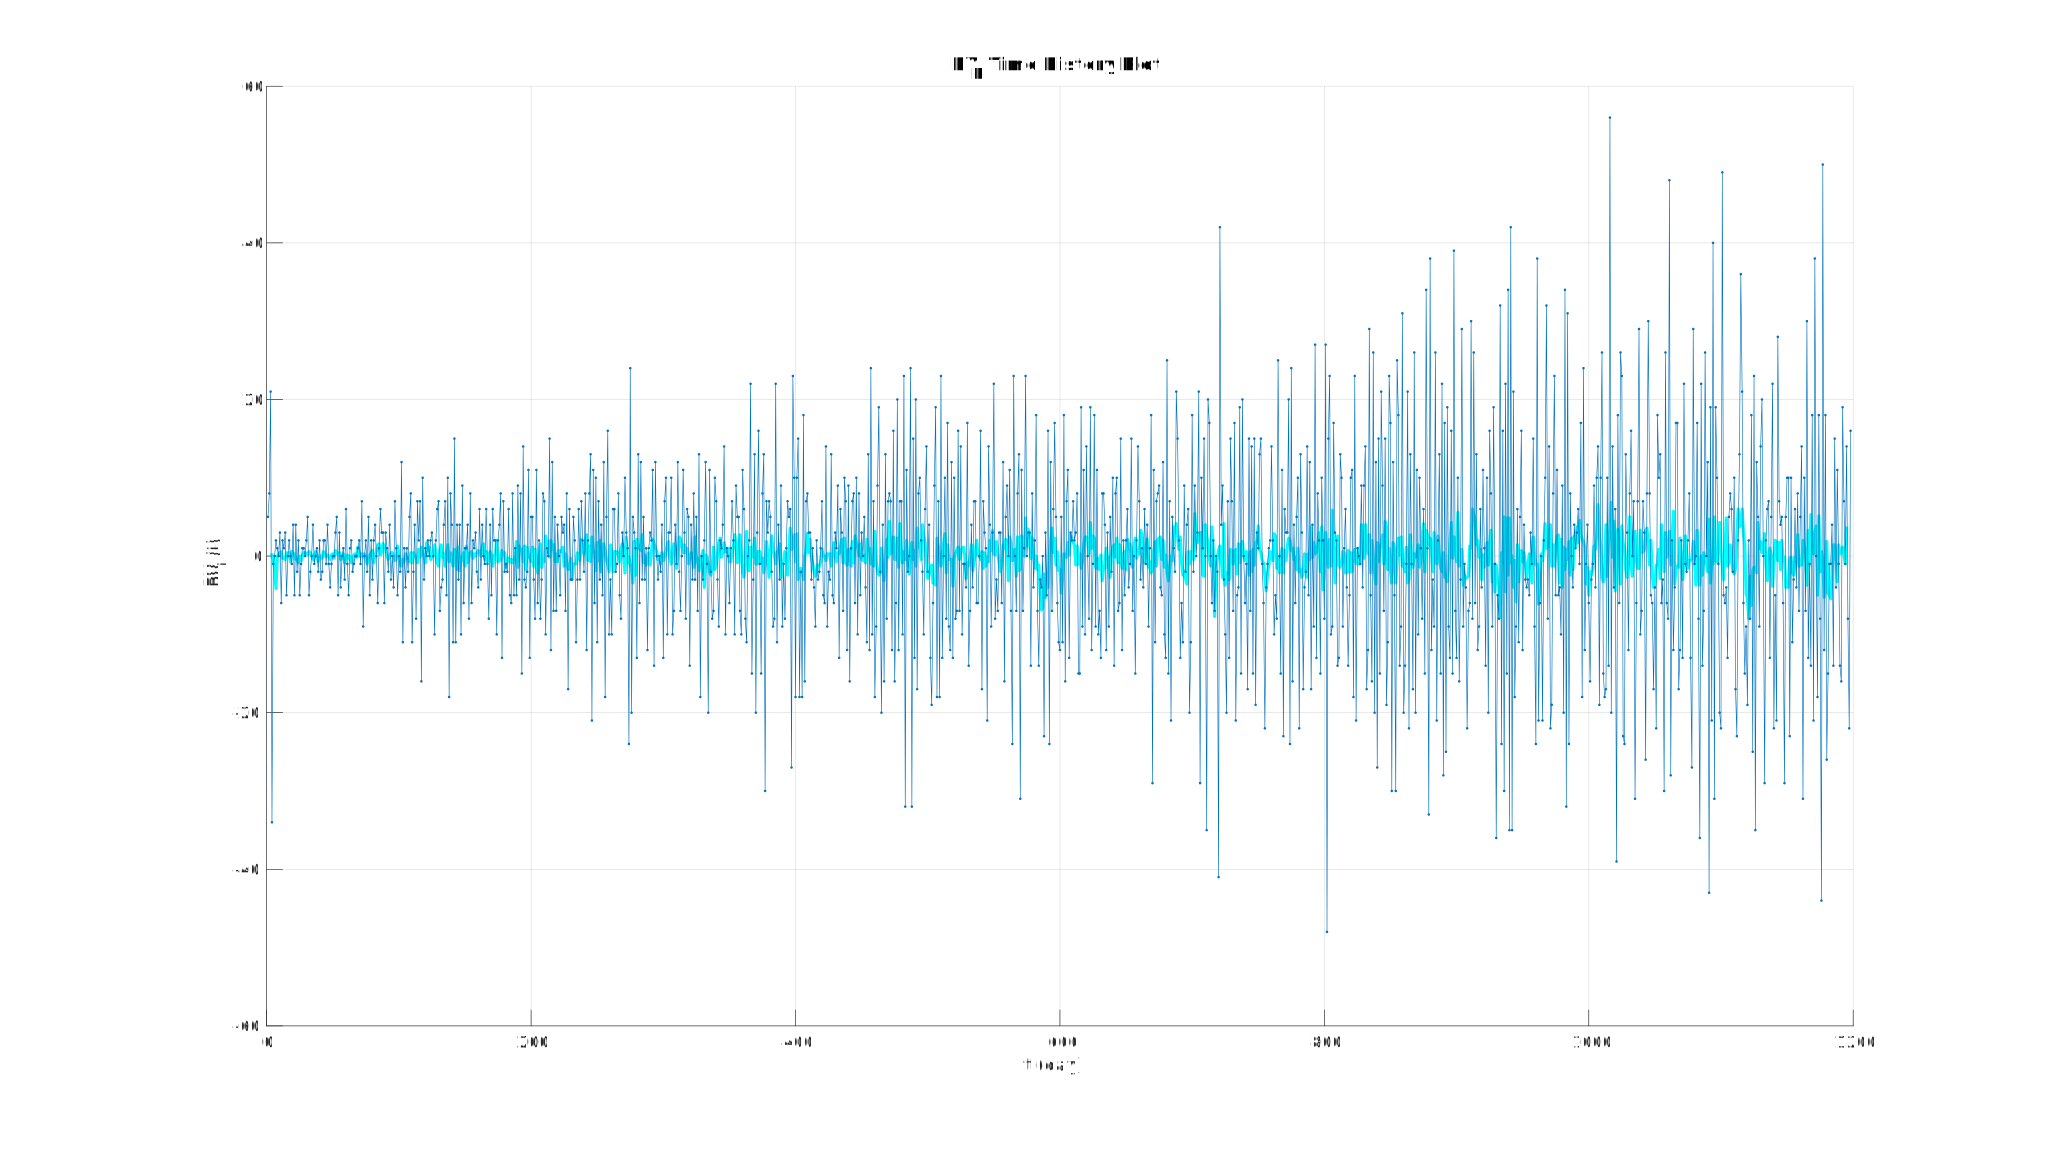
\includegraphics[width=\textwidth]{plots/byb_history.svg.pdf}
        \caption{Διάγραμμα ιστορίας της χρονοσειράς των πρώτων διαφορών, $\{BY_b(t)\}$}
        \label{fig:byb_history}
    \end{center}
\end{figure}

Ο παραπάνω ισχυρισμός περί απαλοιφής τάσης ενισχύεται και από τα ακόλουθα διαγράμματα δειγµατικής αυτοσυσχέτισης και δειγµατικής µερικής αυτοσυσχέτισης της χρονοσειράς των πρώτων διαφορών:

\begin{figure}[H]
    \begin{center}
        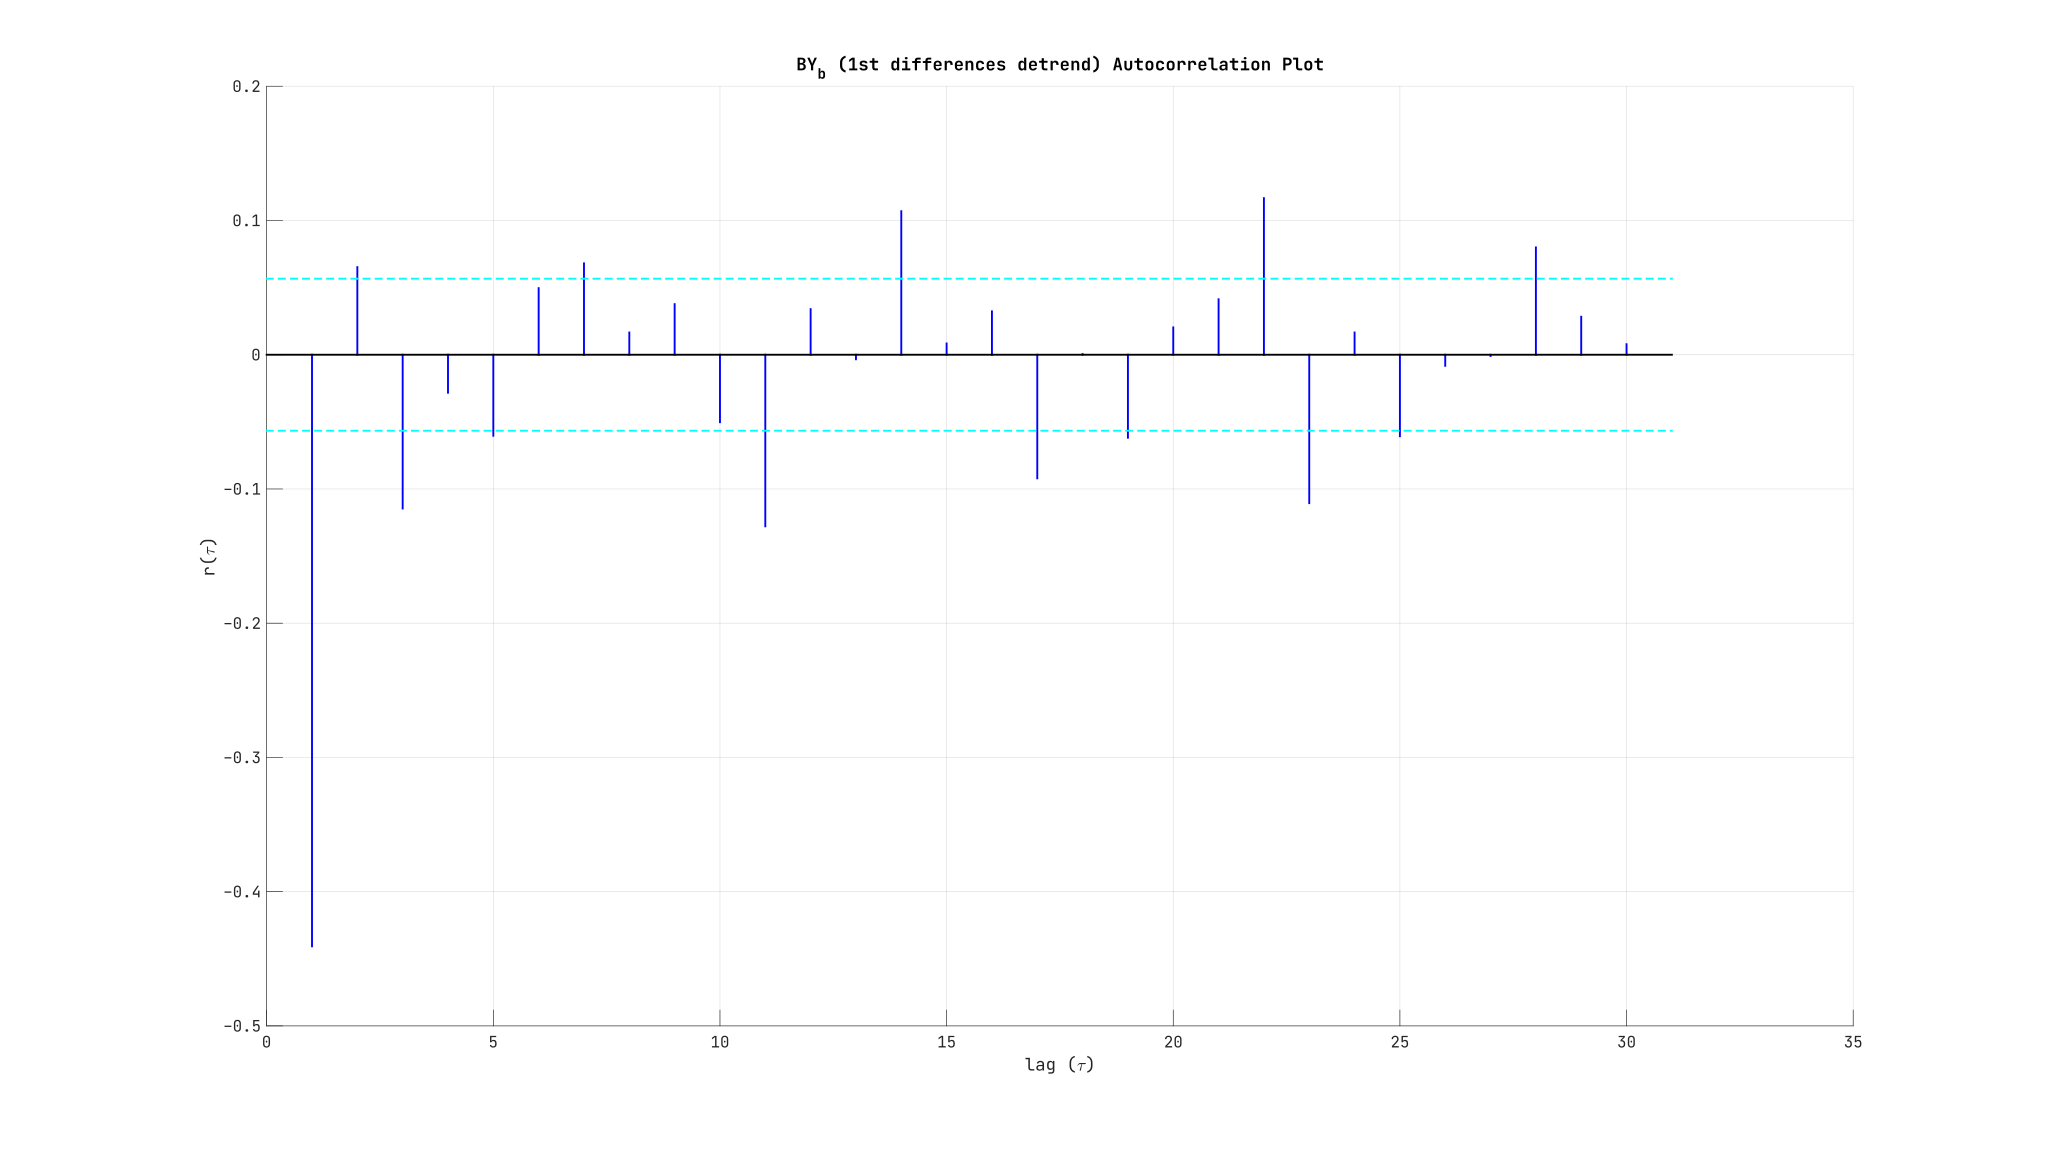
\includegraphics[width=\textwidth]{plots/byb_autocorrelation.svg.pdf}
        \caption{Διάγραμμα (δειγματικής) αυτοσυσχέτισης της χρονοσειράς των πρώτων διαφορών, $r_{BY_b}(\tau)$}
        \label{fig:byb_autocorrelation}
    \end{center}
\end{figure}

\begin{figure}[H]
    \begin{center}
        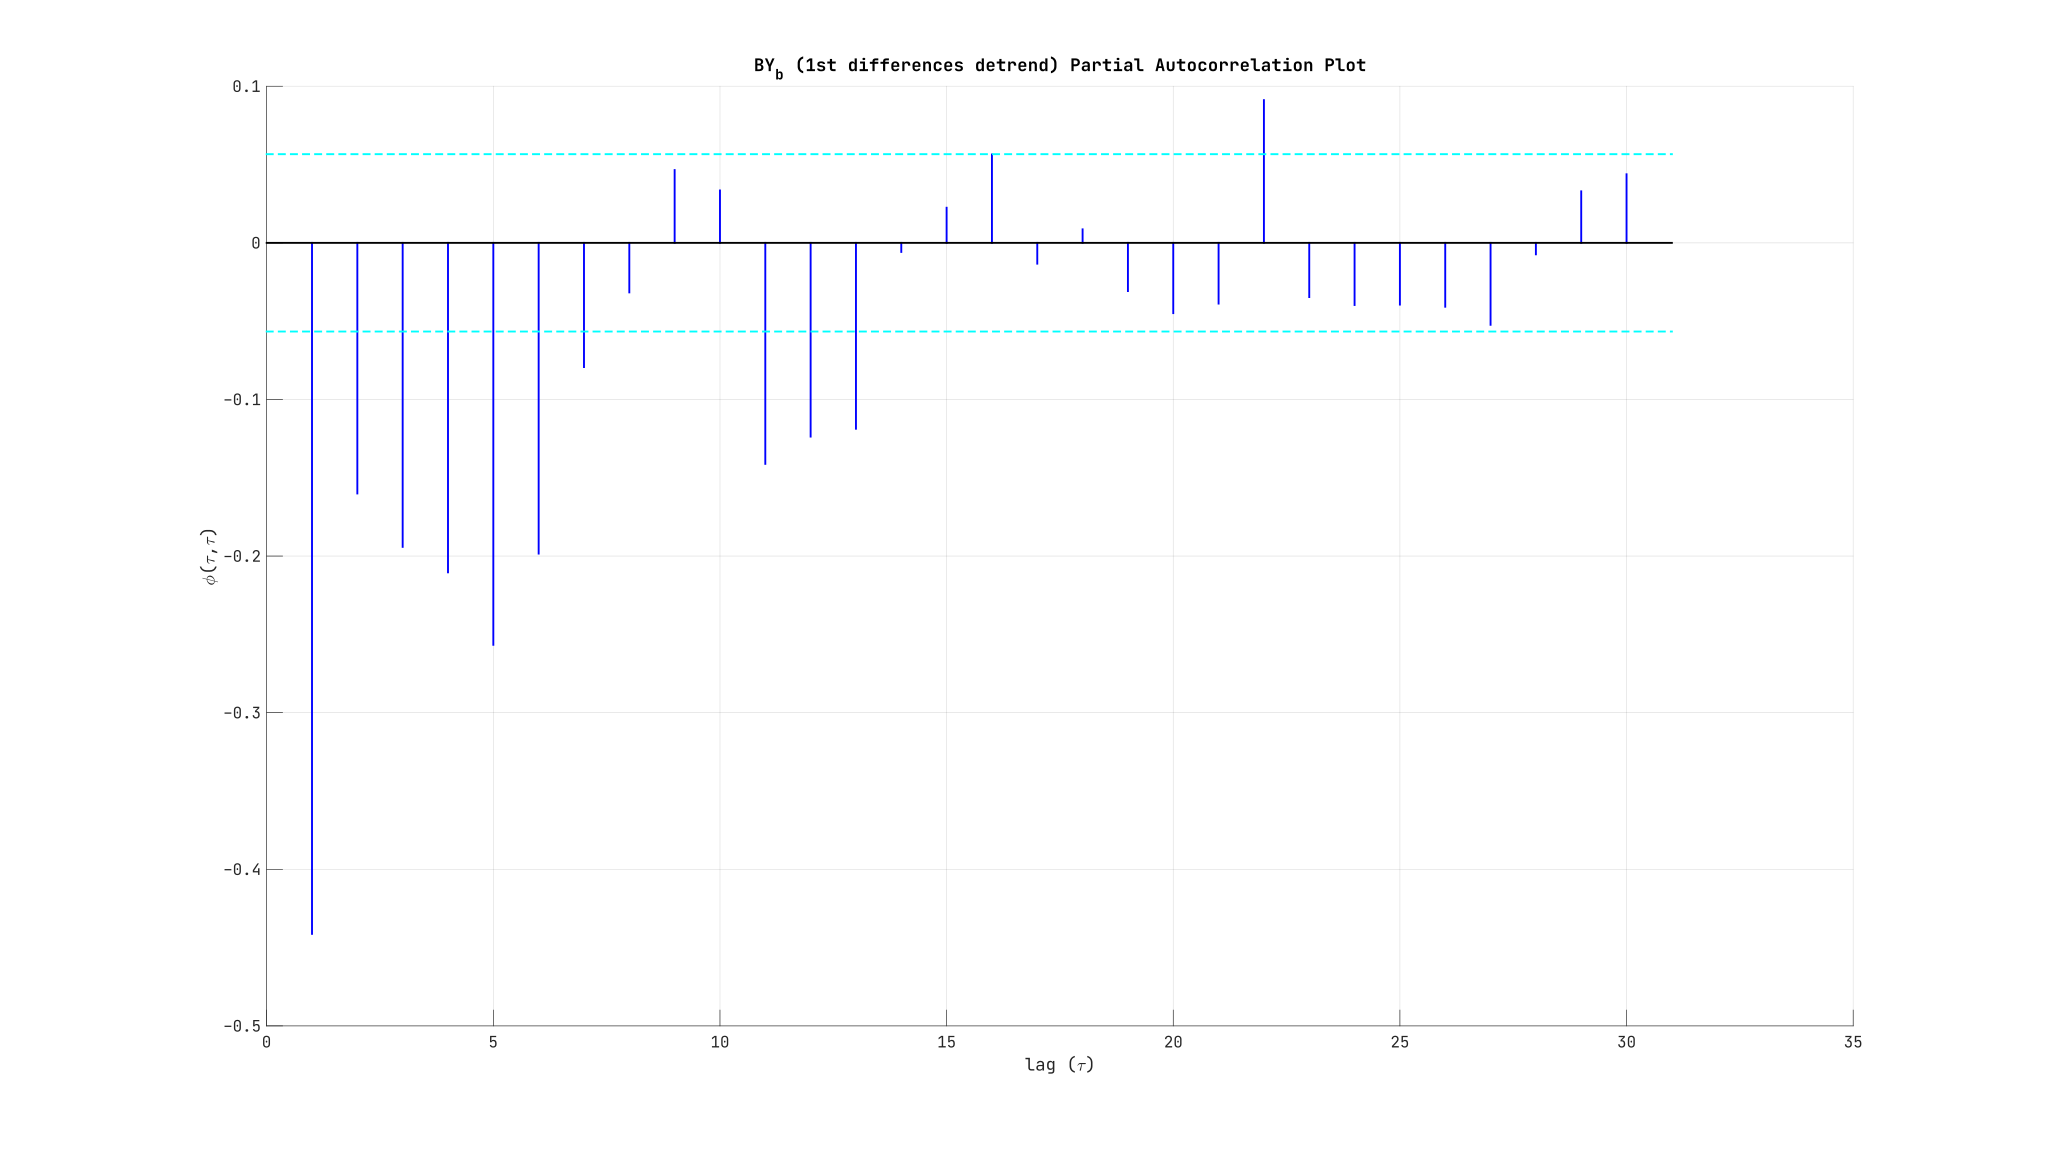
\includegraphics[width=\textwidth]{plots/byb_partial_autocorrelation.svg.pdf}
        \caption{Διάγραμμα (δειγματικής) μερικής αυτοσυσχέτισης της χρονοσειράς των πρώτων διαφορών, $\phi_{BY_b}(\tau)$}
        \label{fig:byb_partial_autocorrelation}
    \end{center}
\end{figure}

όπου αν και δεν φαίνεται η χρονοσειρά να παρουσιάζει αυτοσυσχέτιση λευκού θορύβου επίσης όμως δεν φαίνεται να παρουσιάζει και (στατιστικά) σημαντικές αυτοσυσχετίσεις (σχήμα \ref{fig:byb_autocorrelation}) ή αργή πτώση των τιμών. 

Σε ότι αφορά τη διασπορά της χρονοσειράς των πρώτων διαφορών, επιστρέφοντας στο διάγραμμα ιστορίας της (σχήμα \ref{fig:byb_history}) και συγκρίνοντάς το με το διάγραμμα ιστορίας της αρχικής χρονοσειράς (σχήμα \ref{fig:yb_history}) παρατηρούμε ότι η διασπορά της χρονοσειράς των πρώτων διαφορών φαίνεται να μεταβάλλεται αρκετά σχετικά με την αυξητική \textquote{καμπλύλη} της τάσης της αρχικής χρονοσειράς. Επομένως, είναι αναγκαίο να προσπαθήσουμε να σταθεροποίσουμε τη διασπορά της προκύπτουσας χρονοσειράς αίροντας την εξάρτησή της από τη τάση της αρχικής, κάτι που αναλύεται ακολούθως.

\section{Απαλοιφή Στοχαστικής Τάσης \& Σταθεροποίηση Διασποράς}

Η απαλοιφή της τάσης (\tl{detrending}) θεωρούμε πως έχει επιτευχθεί ικανοποιητικά παίρνοντας τις πρώτες διαφορές στην αρχική χρονοσειρά. Ωστόσο, πριν πάρουμε τις πρώτες διαφορές θα μας ενδιέφερε να απαλείψουμε την εξάρτηση της διασποράς της (αρχικής) χρονοσειράς από τη τάση. Για αυτό θα χρησιμοποιηθεί ο μετασχηματισμός των \tl{Box \& Cox} με $\lambda=0.5$ για τους ίδιους λόγους που εξηγήθηκαν στο βήμα \ref{ch:step1} κατά την επεξεργασία της χρονοσειράς \textquote{\tl{A}}.

Ο μετασχηματισμός, λοιπόν, που χρησιμοποιηθήκε στην αρχική χρονοσειρά \tl{B} είναι αυτός της τετραγωνικής ρίζας. Δηλαδή, αρχικά η $\{Y_b(t)\}$ μετασχηματίστηκε σε:
\begin{align}
    sqrt(Y_b)(t) = \sqrt{Y_b(t)}
\end{align}

Ακολούθως, δίνεται το διάγραμμα ιστορίας (μαζί με το \tl{MA(7) smoothing} όπως έχει αναφερθεί παραπάνω) για τη χρονοσειρά των τετραγωνικών ριζών:

\begin{figure}[H]
    \begin{center}
        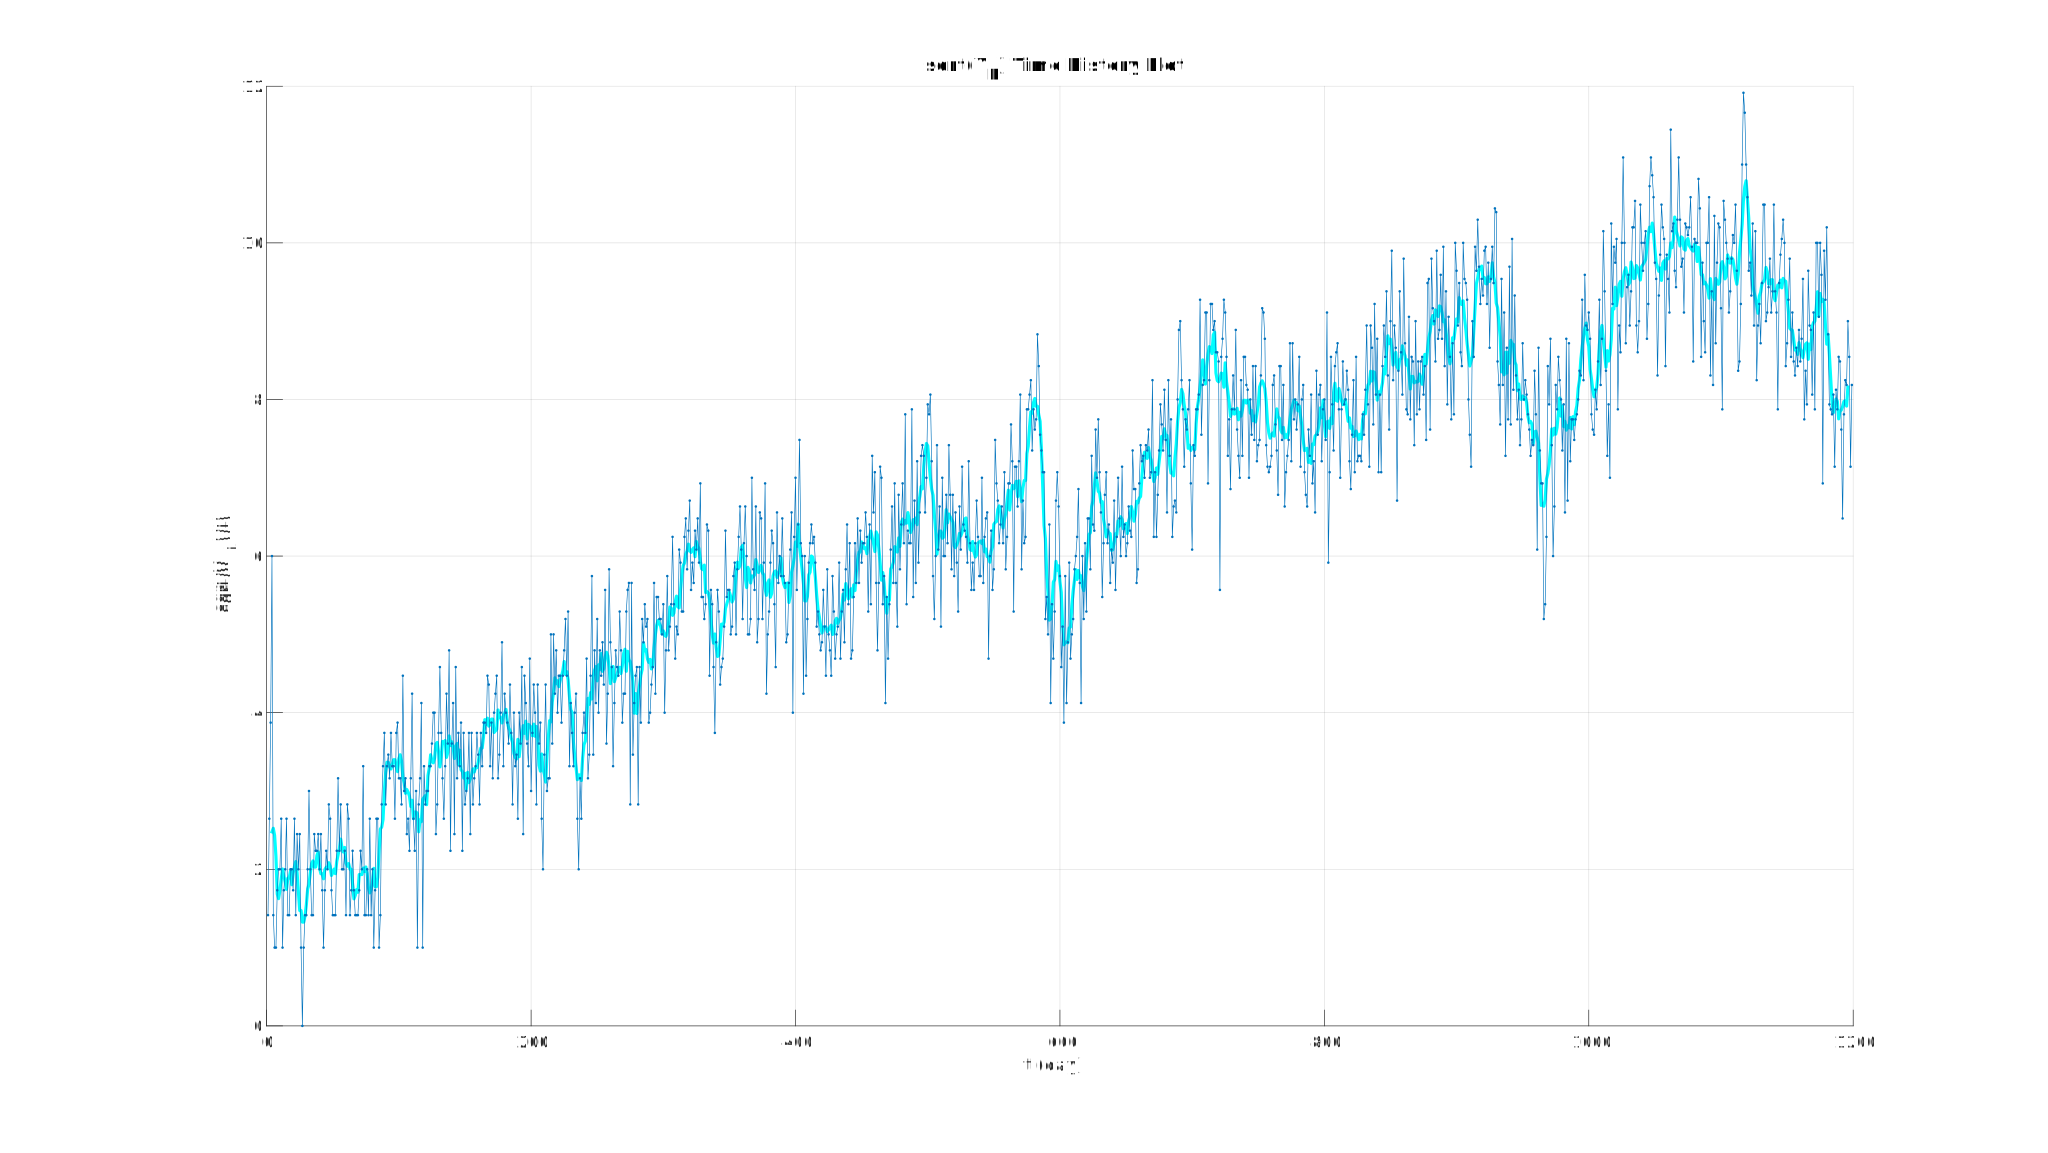
\includegraphics[width=\textwidth]{plots/sqrtyb_history.svg.pdf}
        \caption{Διάγραμμα ιστορίας της χρονοσειράς των τετραγωνικών ριζών, $\{sqrt(Y_b)(t)\}$}
        \label{fig:sqrtyb_history}
    \end{center}
\end{figure}

Στη συνέχεια χρησιμοποίηθηκαν οι πρώτες διαφορές για απαλοιφή της τάσης. Συνολικά, λοιπόν, ο μετασχηματισμός που υλοποιήθηκε για μετασχηματισμό της αρχικής χρονοσειράς σε στάσιμη είναι ο ακόλουθος:
\begin{align}
    X_b(t) = \sqrt{Y_b(t)} - \sqrt{Y_b(t-1)}
\end{align}

με τη χρονοσειρά $\{X_b(t)\}$ να είναι η στάσιμη εκδοχή της $\{Y_b(t)\}$. Παρακάτω, φαίνεται το διάγραμμα ιστορίας της $\{X_b(t)\}$ όπου επιβεβαιώνεται η υπόθεσή μας για συσχέτιση της διασποράς με την τάση (αφού πλέον δεν φαίνεται αυτή η \textquote{κυματοειδής} μεταβολή της διασποράς). Θεωρούμε, δηλαδή, ότι εφαρμόζοντας το μετασχηματισμό της τετραγωνικής ρίζας στην αρχική χρονοσειρά \textbf{πριν} πάρουμε τις πρώτες διαφορές επιτυγχάνουμε την απεξάρτηση της διασποράς από την χρονικής μεταβολή της τάσης. Η χρονοσειρά $\{X_b(t)\}$ λοιπόν που προκύπτει αφενός δεν έχει εξάρτηση της διασποράς από την τάση και αφετέρου η στοχαστική τάση έχει απαλειφθεί.

\begin{figure}[H]
    \begin{center}
        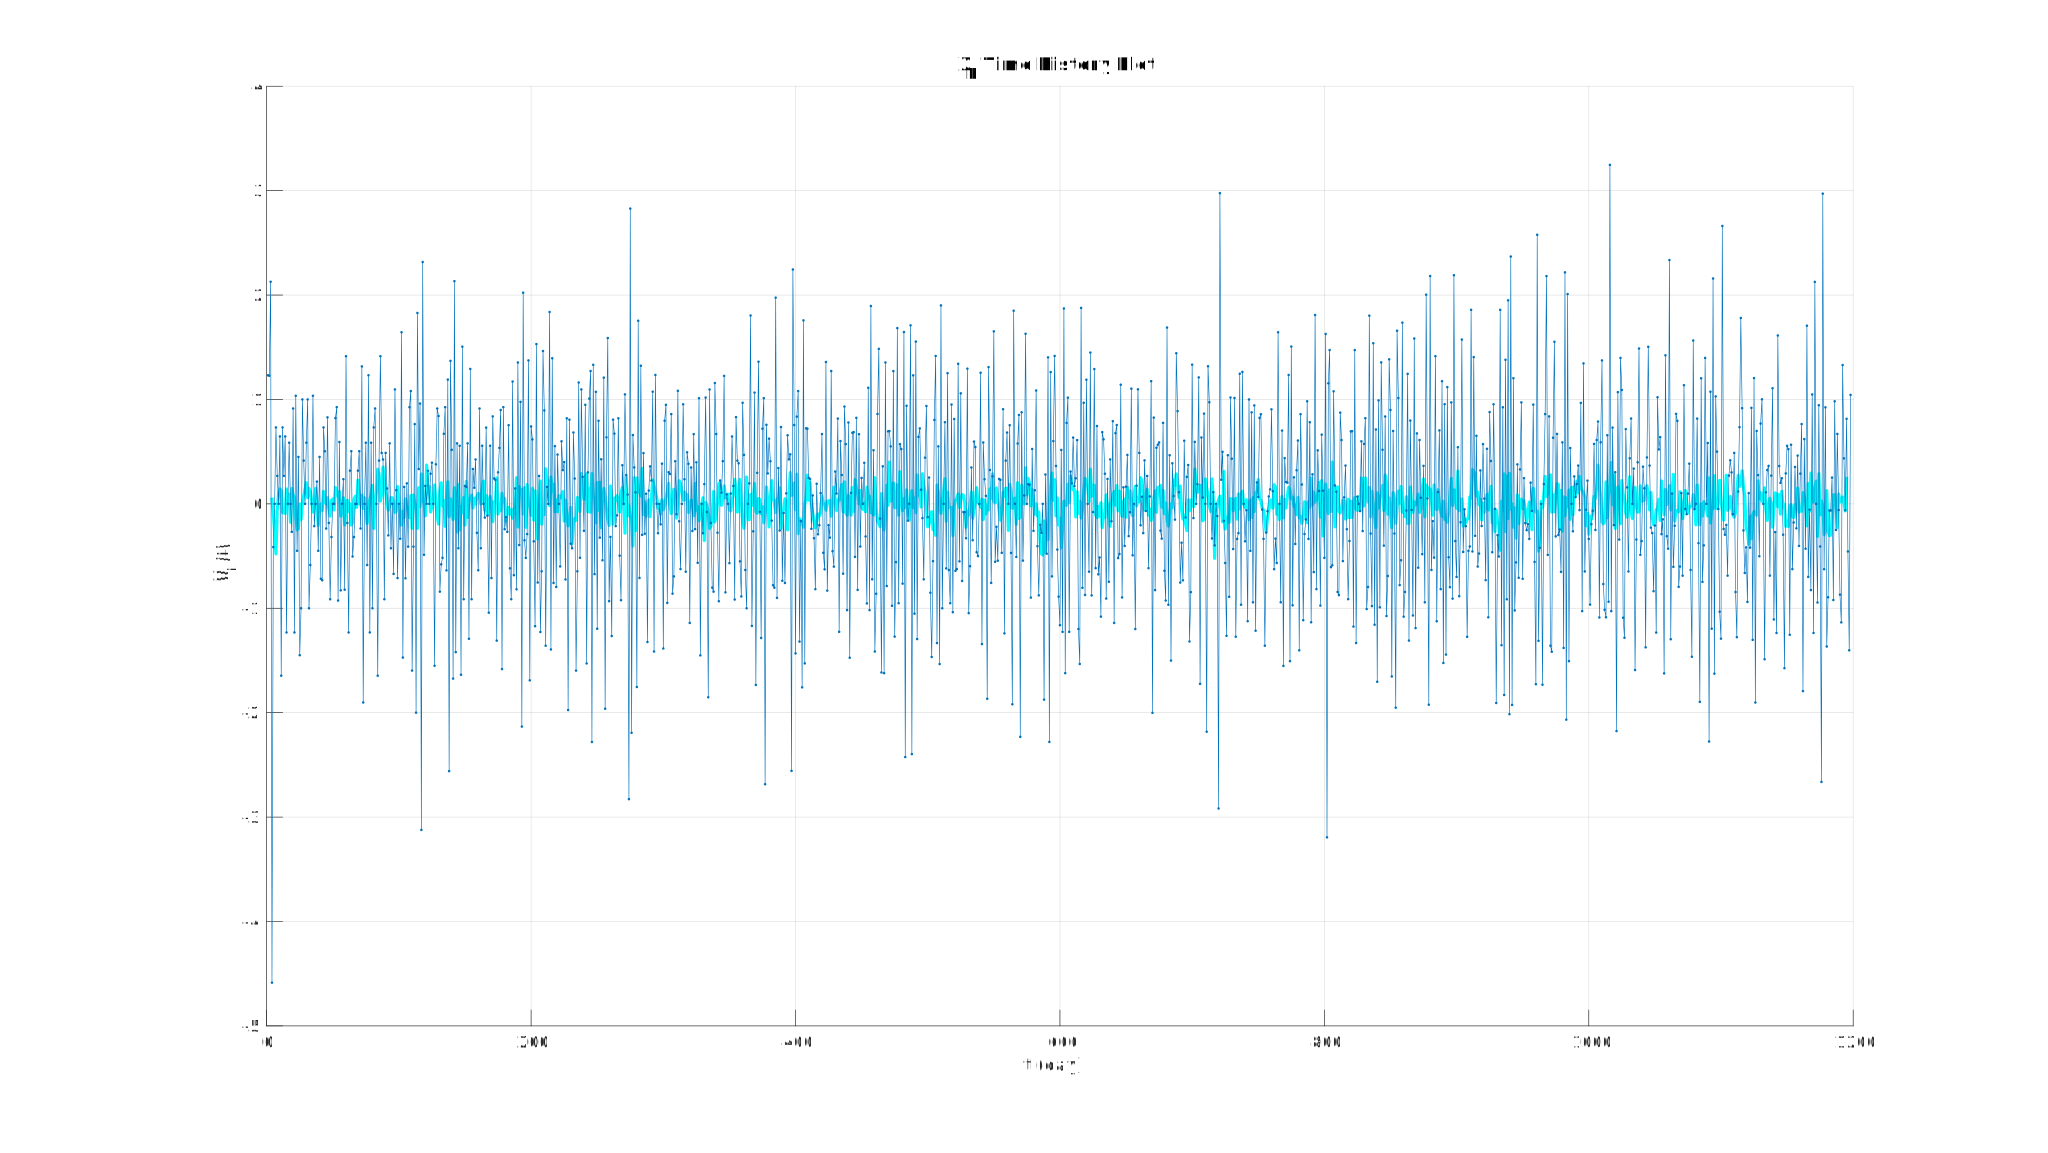
\includegraphics[width=\textwidth]{plots/xb_history.svg.pdf}
        \caption{Διάγραμμα ιστορίας της στάσιμης χρονοσειράς, $\{X_b(t)\}$, ως οι πρώτες διαφορές των τετραγωνικών ριζών της αρχικής χρονοσειράς}
        \label{fig:xb_history}
    \end{center}
\end{figure}

Για τη χροοσειρά των πρώτων διαφορών των τετραγωνικών ριζών που καταλήξαμε, παραθέτονται επίσης και τα διαγράμματα δειγματικής αυτοσυσχέτισης και δειγματικής μερικής αυτοσυσχέτισης με τα όρια σημαντικότητας (για εμπιστοσύνη 95\%):

\begin{figure}[H]
    \begin{center}
        \includegraphics[width=\textwidth]{plots/xb_autocorrelation.svg.pdf}
        \caption{Διάγραμμα (δειγματικής) αυτοσυσχέτισης της στάσιμης χρονοσειράς, $r_x(\tau)$}
        \label{fig:xb_autocorrelation}
    \end{center}
\end{figure}

\begin{figure}[H]
    \begin{center}
        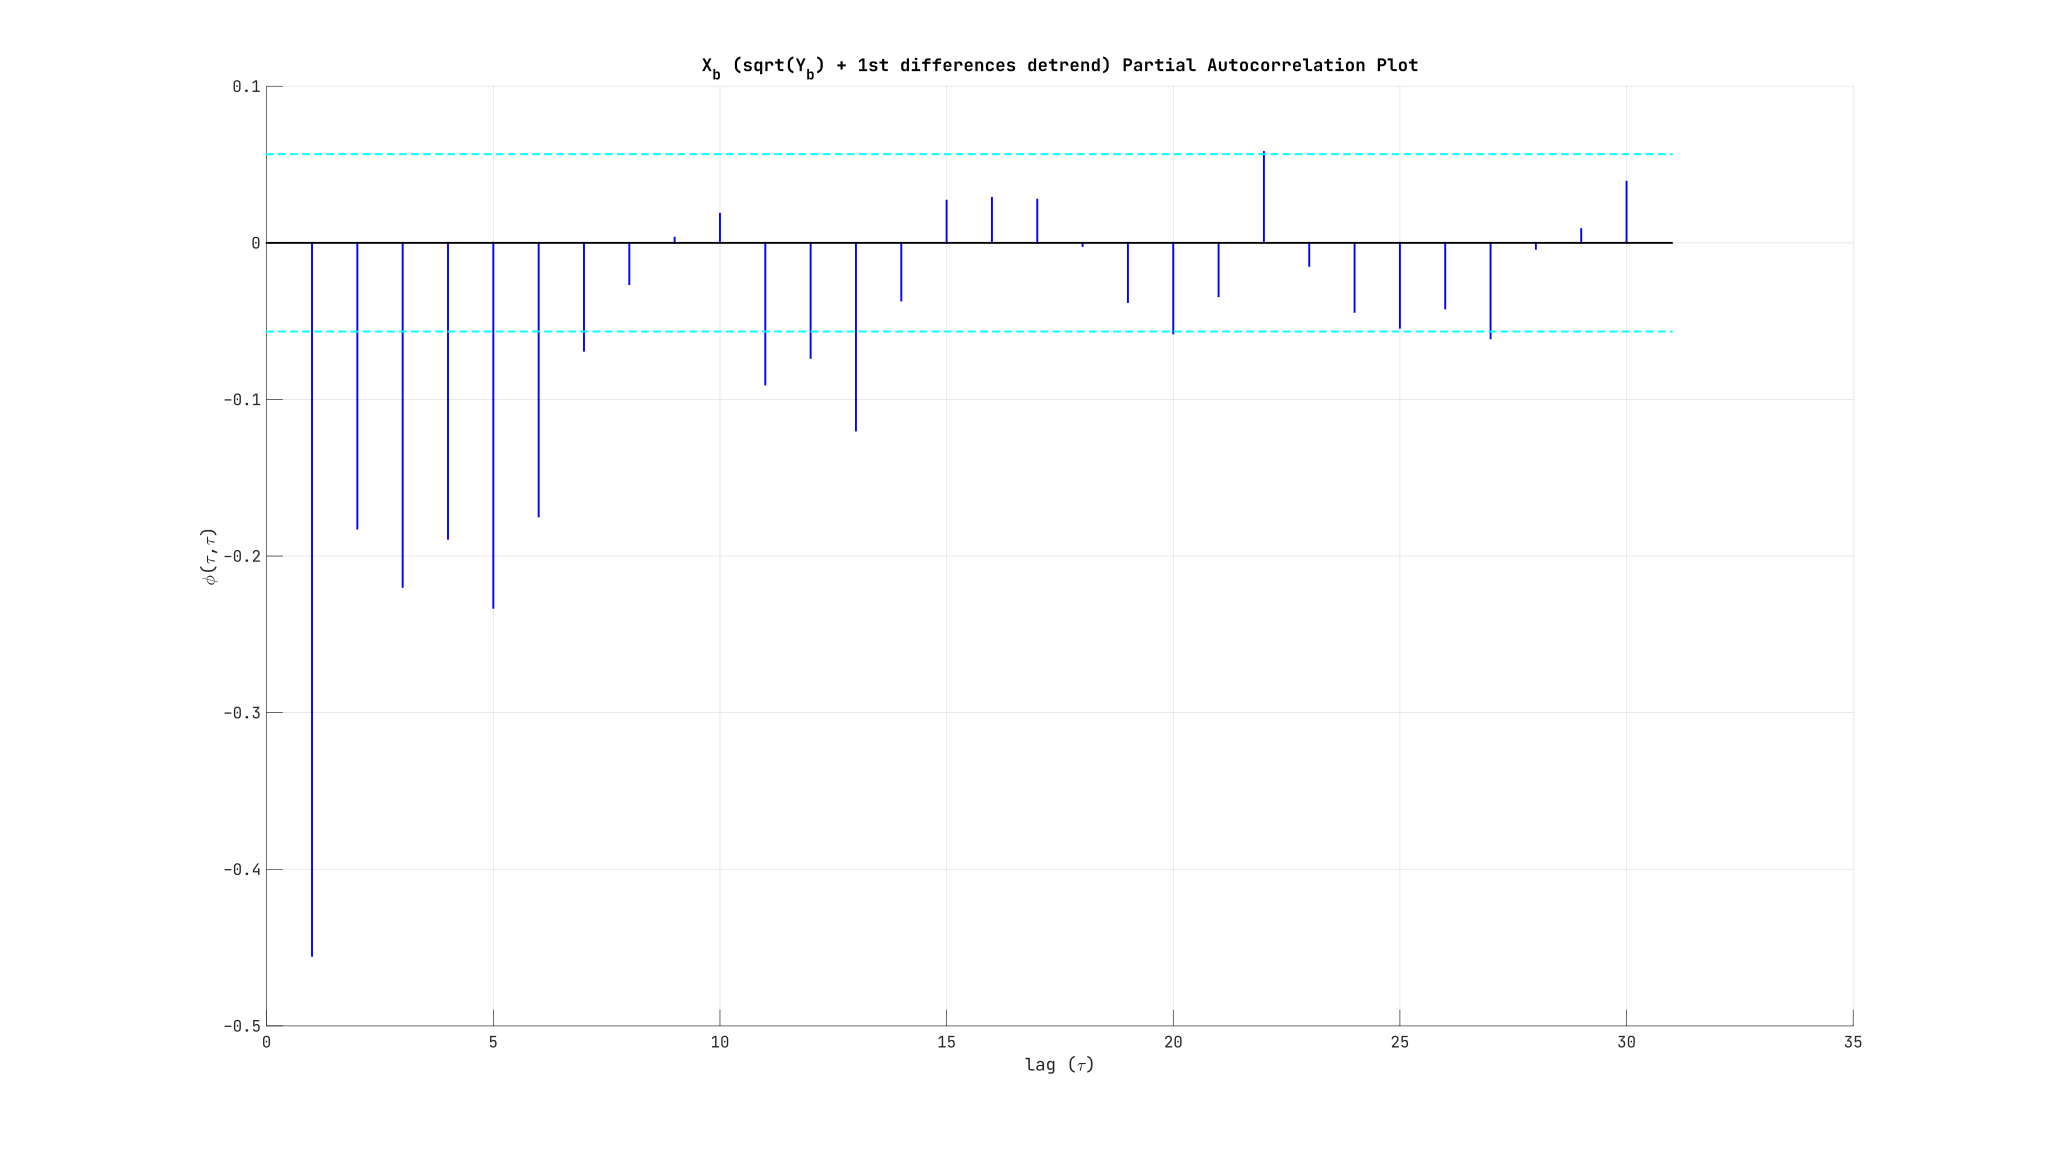
\includegraphics[width=\textwidth]{plots/xb_partial_autocorrelation.svg.pdf}
        \caption{Διάγραμμα (δειγματικής) μερικής αυτοσυσχέτισης της στάσιμης χρονοσειράς, $\phi_x(\tau)$}
        \label{fig:xb_partial_autocorrelation}
    \end{center}
\end{figure}

τα οποία όπως είναι αναμενόμενο είναι σχεδόν ίδια με τα αντίστοιχα διαγράμματα της χρονοσειράς μόνο των πρώτων διαφορών (χωρίς δηλαδή το μετασχηματισμό της τετραγωνικής ρίζας), που δόθηκαν στα σχήματα \ref{fig:byb_autocorrelation} και \ref{fig:byb_partial_autocorrelation} παραπάνω.

\par Από το νέο διάγραμμα αυτοσυσχέτισης της $\{X_b(t)\}$ (σχήμα \ref{fig:xb_autocorrelation}) φαίνετα, ωστόσο, ότι μάλλον υπάρχει κάποιος περιοδικός όρος στη χρονοσειρά, ή εποχικότητα, κάτι που έρχεται σε αντίθεση με τον ισχυρισμό μας περί στασιμότητας. Βλέποντας τις \textquote{κορυφές} στο συγκεκριμένο διάγραμμα για υστερήσεις 14 και 28 ημερών να ξεπερνούν τα όρια σημαντικότητας και άρα να είναι (στατιστικά) μη-μηδενικές, μπορούμε να συμπεράνουμε πως στις προβολές του βίντεο \tl{B} μάλλον υπάρχει κάποιος εποχικός όρος διάρκειας 14 ημερών, τον οποίο θα προσπαθήσουμε να απαλείψουμε ακολούθως. 

\section{Εκτίμηση \& Απαλοιφή Εποχικότητας}
\label{sec:step3-deseason}

\subsection{Εκτίμηση Εποχικού Όρου}

Αρχικά θα πρέπει να εκτιμήσουμε τον περιοδικό όρο της $\{X_b(t)\}$ διάρκειας 14 ημερών. Υποθέτουμε, δηλαδή πως η $\{X_b(t)\}$ γράφεται ως εξής:
\begin{align}
    X_b(t) = X_{b_{deseasoned}}(t) + \widetilde{s_b}(t)
    \label{eq:xb=xb_ds+sb}
\end{align}

όπου η $\widetilde{s_b}$ είναι περιοδική ακολουθία διάρκειας 14 ημερών. Χρησιμοποιήθηκε η μέθοδος του μέσου όρου των στοιχειών της περιοδικής ακολουθίας για την εύρεση του εποχικού όρου. Έτσι, θα είναι:
\begin{align}
    \left(\widetilde{s_b}\right)_i = \frac{1}{85} \sum_{j=0}^{84} \left(x_b\right)_{i+14j} , \ \ \  i=1,..,14
    \label{eq:sb_ι}
\end{align}

καθώς υπάρχουν 85 περίοδοι στα 1198 δείγματα της $\{X_b(t)\}$ με μήκος περιόδου 14 δείγματα (ή εποχικότητα 14 ημερών στην αρχική χρονοσειρά προβολών του βίντεο \tl{B}). Η πρώτη περίοδος του εποχικού όρου $\widetilde{s_b}$ φαίνεται στο ακόλουθο διάγραμμα:

\begin{figure}[H]
    \begin{center}
        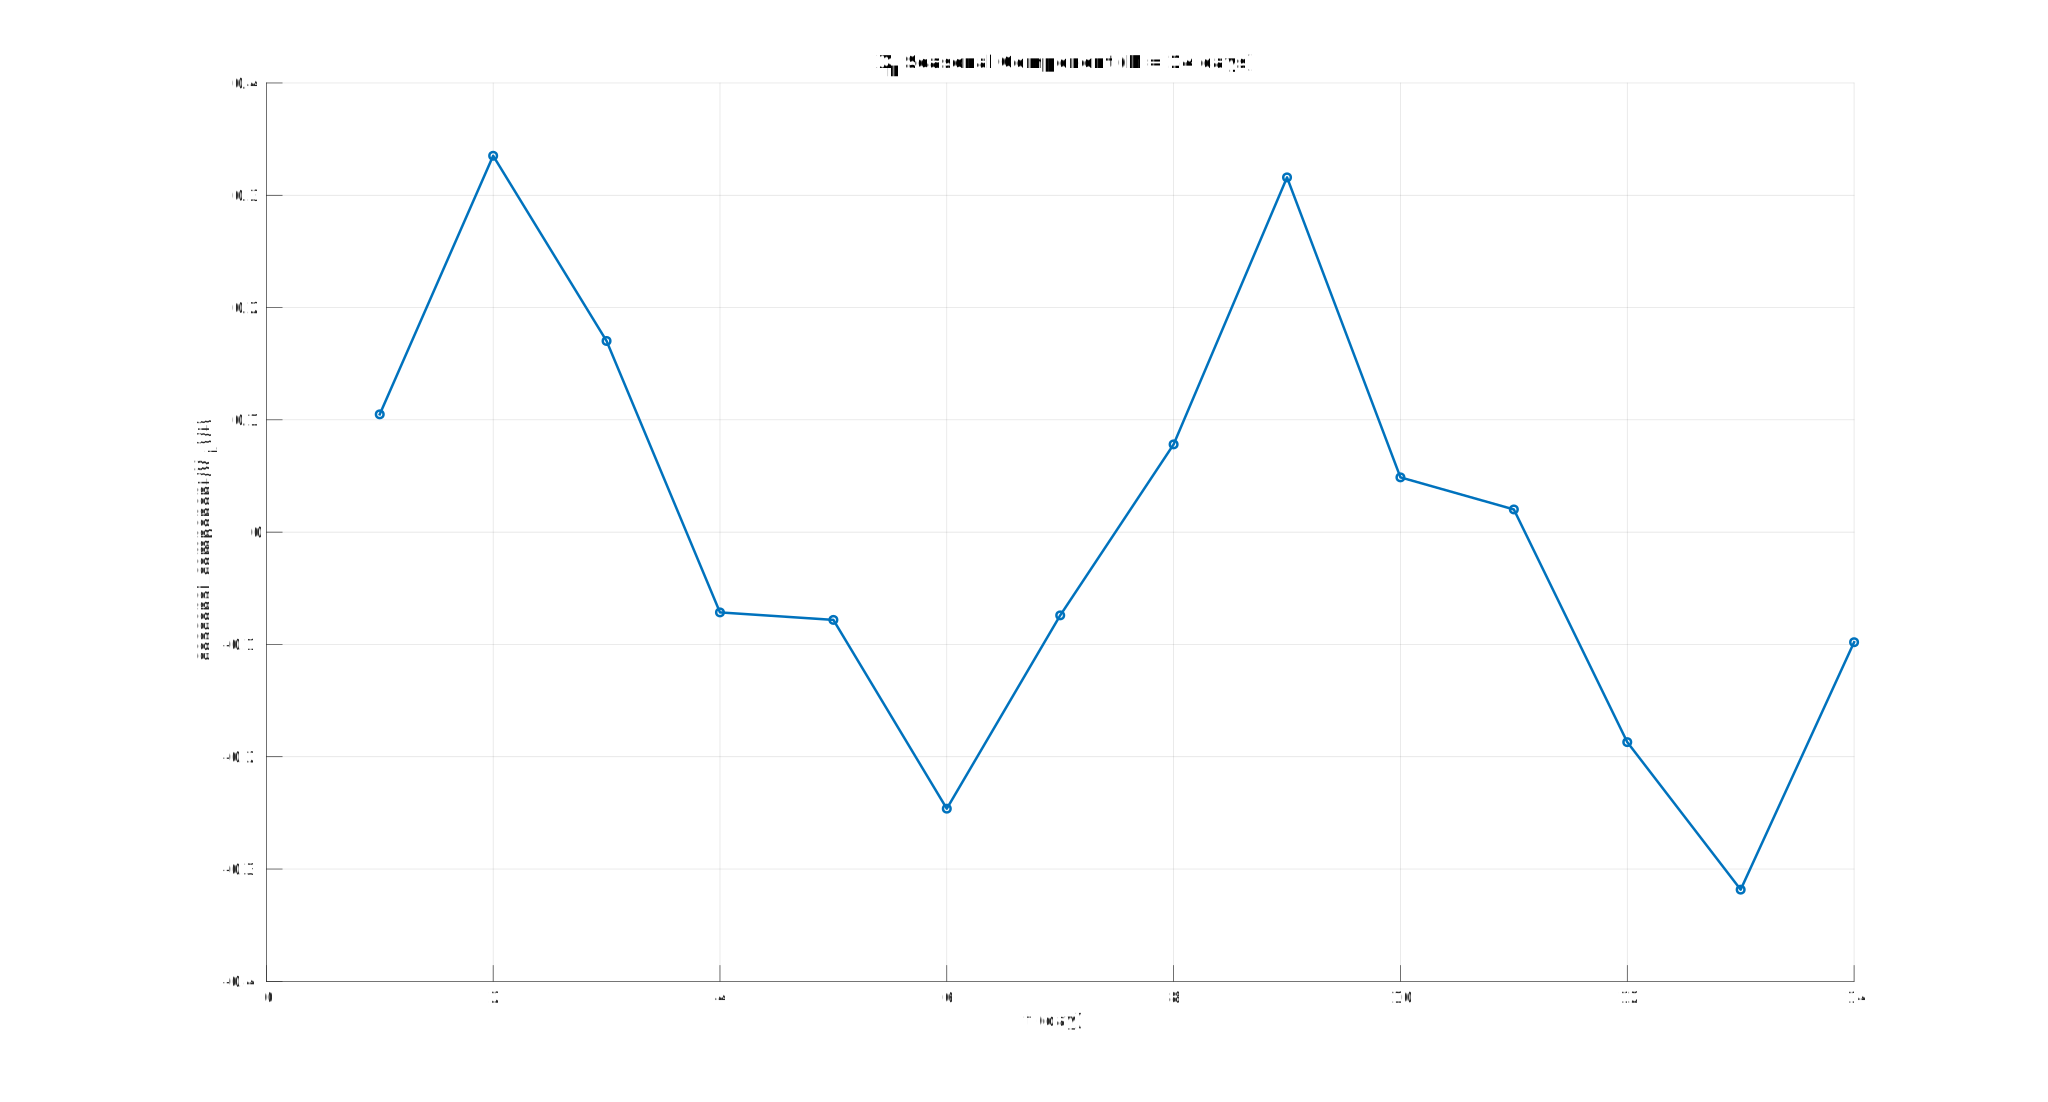
\includegraphics[width=\textwidth]{plots/xb_seasonal_component.svg.pdf}
        \caption{Πρώτη περίοδος του εποχικού όρου της $\{X_b(t)\}$, $\widetilde{s_b}$}
        \label{fig:xb_seasonal_component}
    \end{center}
\end{figure}

\subsection{Απαλοιφή Εποχικού Όρου}

Για την απαλοιφή του εποχικού όρου που εκτιμήθηκε παραπάνω, αφαιρέθηκε κάθε τιμή της περιοδικής ακολουθίας της σχέσης (\ref{eq:sb_ι}) από το αντίστοιχο δείγμα της $\{X_b(t)\}$,
δίνοντας την χρονοσειρά χωρίς εποχικότητα, $\{X_{b_{deseasoned}}(t)\}$:
\begin{align}
    X_{b_{deseasoned}}(t) = X_b(t) - \widetilde{s_b}(t)
    \label{eq:xb_ds_t}
\end{align}

\par Παρακάτω, παρατίθενται για την τελευταία τα διαγράμματα ιστορίας, δειγματικής αυτοσυσχέτισης και δειγματικής μερικής αυτοσυσχέτισης:

\begin{figure}[H]
    \begin{center}
        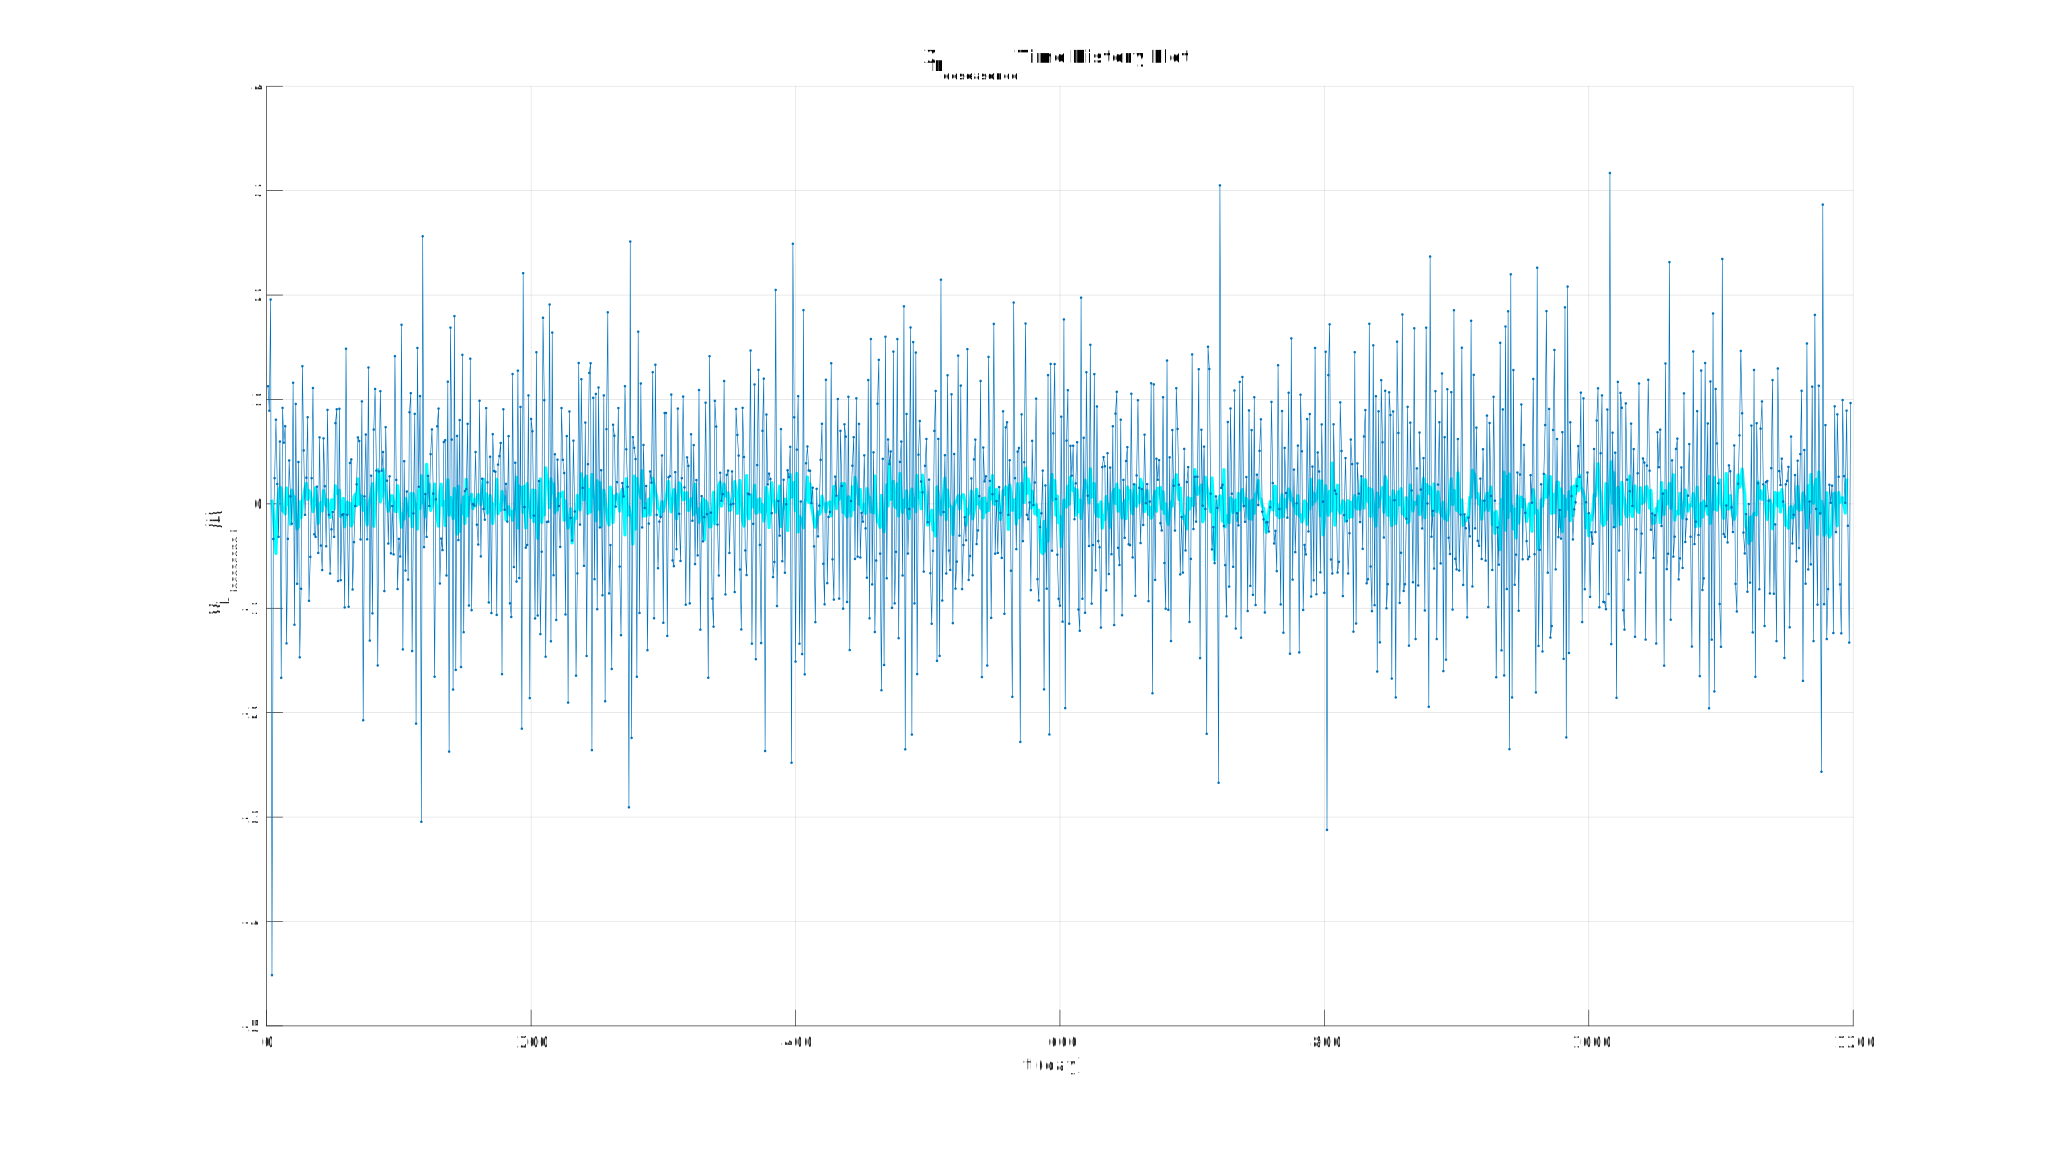
\includegraphics[width=\textwidth]{plots/xb_deseasoned_history.svg.pdf}
        \caption{Διάγραμμα ιστορίας της χρονοσειράς $\{X_b(t)\}$ απαλλαγμένης από εποχικότητα, $\{X_{b_{deseasoned}}(t)\}$}
        \label{fig:xb_deseasoned_history}
    \end{center}
\end{figure}

\begin{figure}[H]
    \begin{center}
        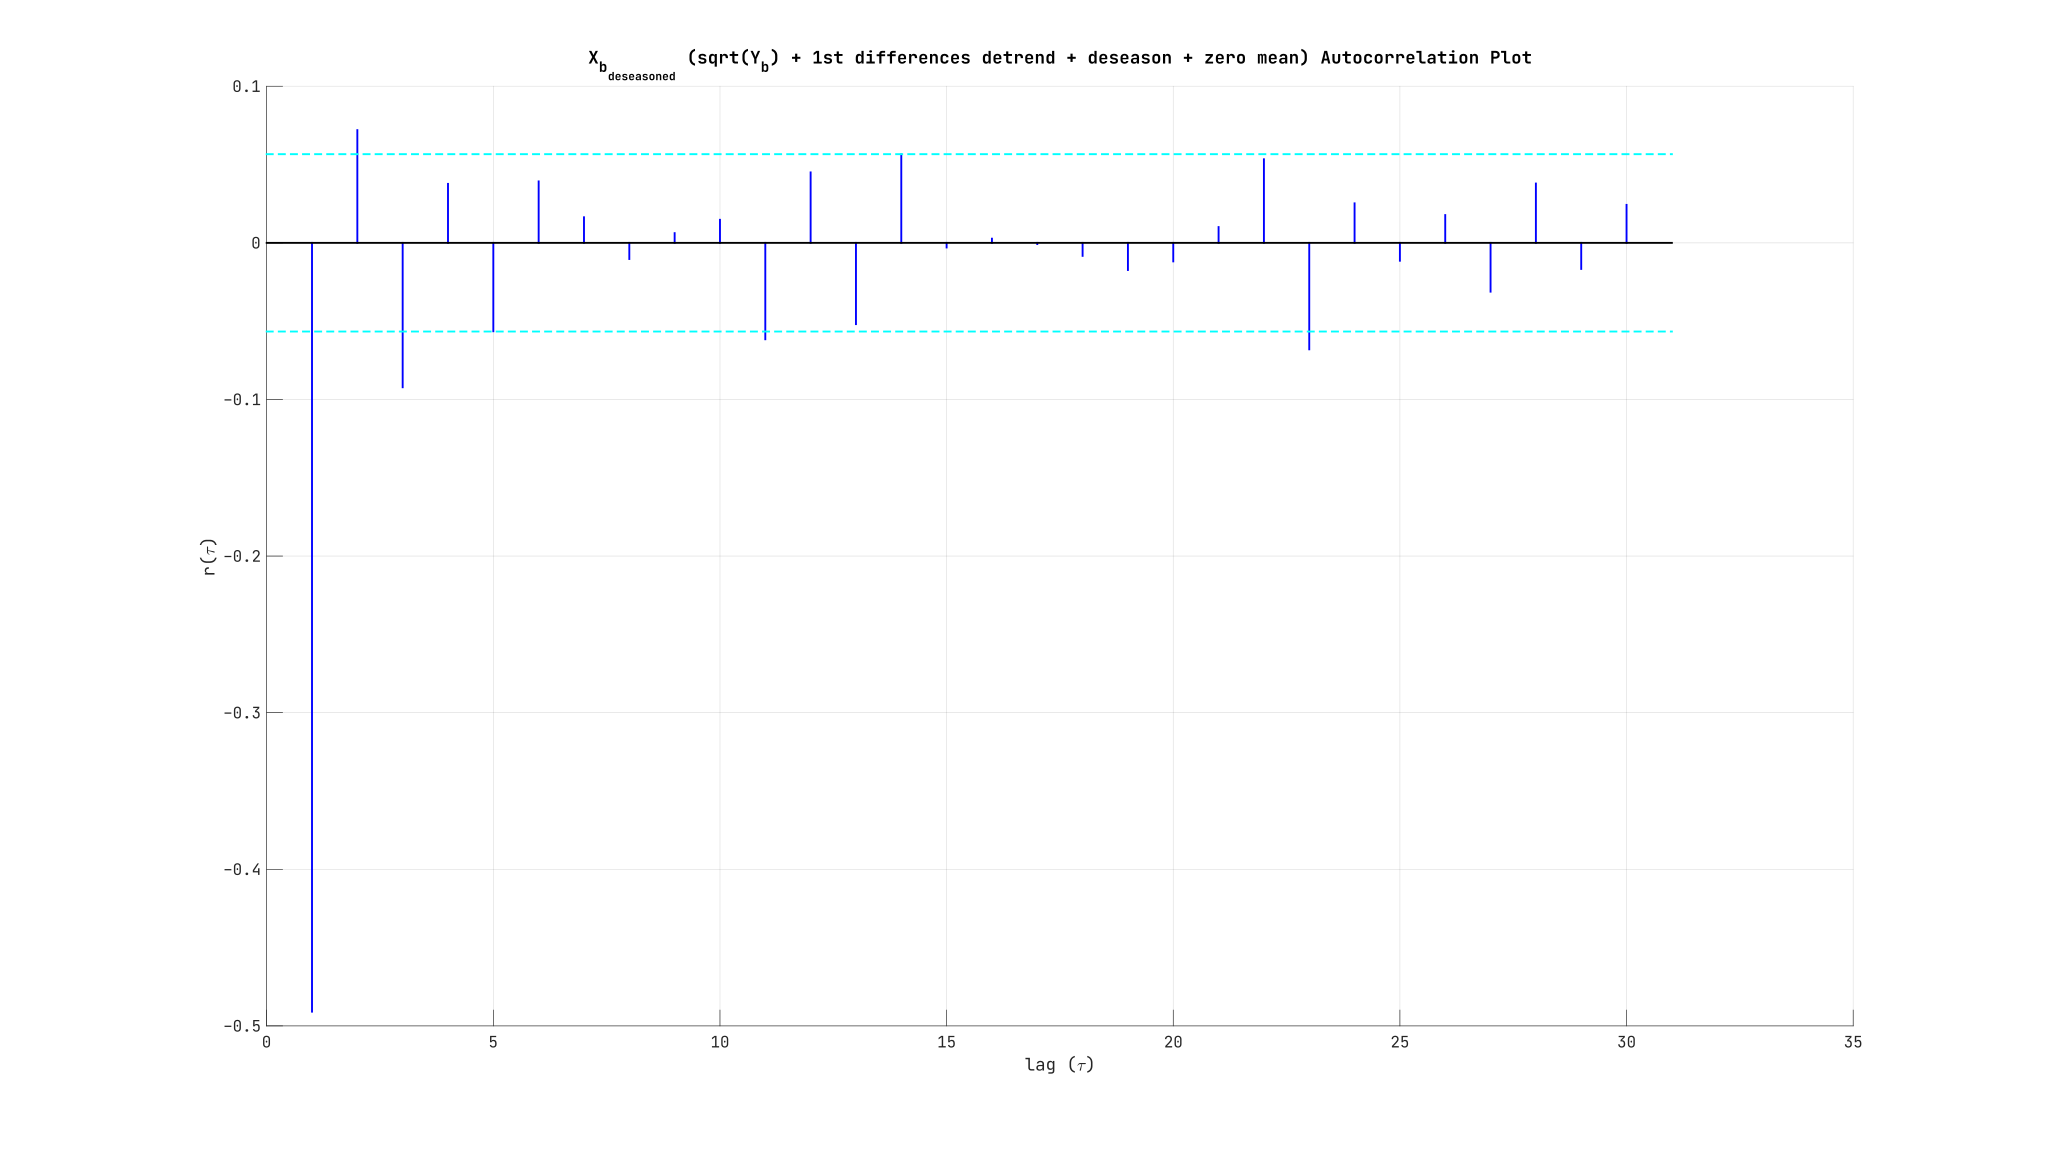
\includegraphics[width=\textwidth]{plots/xb_deseasoned_autocorrelation.svg.pdf}
        \caption{Διάγραμμα (δειγματικής) αυτοσυσχέτισης της απαλλαγμένης από εποχικότητα χρονοσειράς, $r_x(\tau)$}
        \label{fig:xb_deseasoned_autocorrelation}
    \end{center}
\end{figure}

\begin{figure}[H]
    \begin{center}
        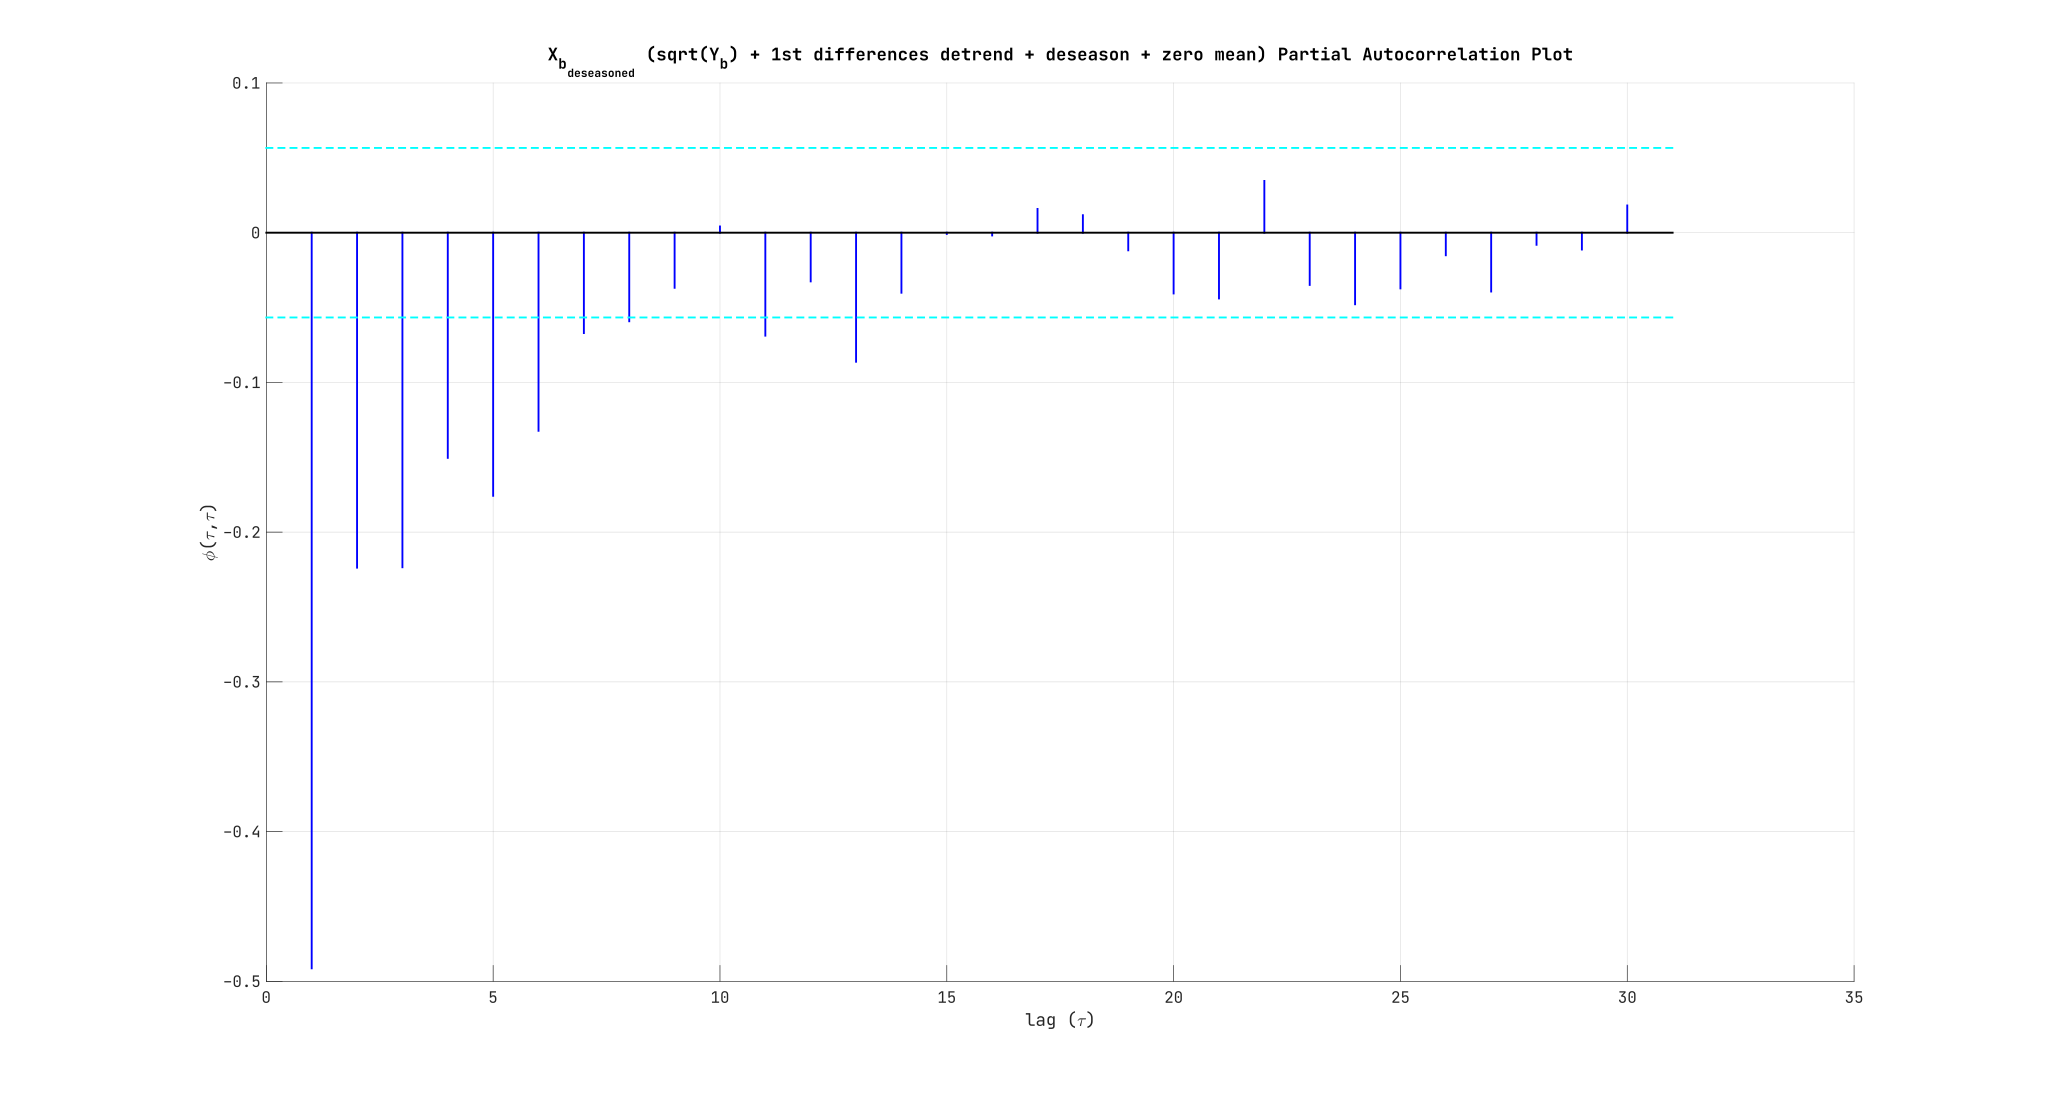
\includegraphics[width=\textwidth]{plots/xb_deseasoned_partial_autocorrelation.svg.pdf}
        \caption{Διάγραμμα (δειγματικής) μερικής αυτοσυσχέτισης της απαλλαγμένης από εποχικότητα χρονοσειράς, $\phi_x(\tau)$}
        \label{fig:xb_deseasoned_partial_autocorrelation}
    \end{center}
\end{figure}

Από τα παραπάνω διαγράμματα και ειδικά από το διάγραμμα της αυτοσυσχέτισης (σχήμα \ref{fig:xb_deseasoned_autocorrelation}) φαίνεται πως αφενός ο εποχικός όρος έχει απαλειφθεί και αφετέρου έχουν μειωθέι και άλλες \textquote{κορυφές} της συνάρτησης αυτοσυσχέτισης της απαλλαγμένης από εποχικότητα χρονοσειράς. 

\subsection{Σύνοψη Διαδικασίας}

\par Καταλήγουμε επομένως στα εξής για τη χρονοσειρά προβολών του βίντεο \tl{B}:\\
Παίρνοντας τις τετραγωνικές ρίζες των τιμών τη αρχικής χρονοσειράς σταθεροποιείται η διασποσρά. Ακολούθως, παίρνουμε πρώτες διαφορές στη χρονοσειρά των τετραγωνικών ριζών και έτσι απαλείφεται η στοχαστική τάση. Από το διάγραμμα αυτοσυσχέτισης της τελευταίας παρατηρούμε την ύπαρξη εποχικότητας με περίοδο 14 ημερών. Ακολούθως εκτιμούμε και απαλείφουμε τον εποχικό όρο, καταλήγοντας έτσι στην $\{X_{b_{deseasoned}}(t)\}$, σχέση (\ref{eq:xb_ds_t}). Αυτή είναι η \textbf{στάσιμη} εκδοχή της $\{Y_b(t)\}$ στην οποία θα προσαρμόσουμε γραμμικό μοντέλο τύπου \tl{ARMA}, όπως αναλύεται στην επόμενη ενότητα.


%-------------------------------------------------------------------------------


\section{Προσαρμογή \tl{ARMA(p,q)}}

Σε αντιστοιχία με τη διαδικασία που ακουλήθηκε κατά τη προσαρμογή γραμμικού μοντέλου στη χρονοσειρά \tl{A}, θα επιχειρήσουμε εδώ τη προσαρμογή μοντέλου \tl{ARMA} και στη χρονοσειρά \tl{B}.

Έτσι, συνεχίζοντας την ανάλυση από το τέλος της ενότητας \ref{sec:step3-deseason}, μετά την εφαρμογή των πρώτων διαφορών στη χρονοσειρά των τετραγωνικών ριζών και την απαλειφή του εποχικού όρου, έχουμε υλοποιήσει το πρώτο στάδιο προσαρμογής ενός μοντέλου \tl{ARIMA(p,d,q)} που είναι η εφαρμογή διαφορών \tl{d}-οστής (στη απαλλαγμένη από εποχικότητα χρονοσειρά). Άρα εδώ θα είναι $d=1$ και η (στάσιμη )χρονοσειρά που καταλήγουμε είναι η $\{X_{b_{deseasoned}}(t)\}$.\\
Το δεύτερο στάδιο είναι η εύρεση των παραμέτρων του μοντέλου \tl{ARMA(p,q)} που θα προσαρμοστεί στη στάσιμη χρονοσειρά, κάτι που αναλύεται στην επόμενη υπο-ενότητα. 

\subsection{Προσαρμογή \tl{ARMA(p,q)} στη στάσιμη χρονοσειρά}

Οι παράμετροι \tl{p} και \tl{q} είναι \tl{hyperparameters} του μοντέλου και επομένως το πρώτο μας μέλημα είναι να βρούμε το βέλτιστο συνδυσμό των παραμέτρων αυτών ή τάξεων του μοντέλου. Προς το σκοπό αυτό θα κάνουμε \tl{grid search} για τιμές των τάξεων από 0 (απουσία του αντίστοιχου όρου) έως και 10.\par

Για την αξιολόγηση του κάθε συνδυασμού χρησιμοποιήθηκαν τα κριτήρια πληροφορίας \tl{Akaike (AIC)} και \tl{Forward Prediction Error (FPE)}, όπως αυτά ορίστηκαν στις σχέσεις (\ref{eq:aic}) και (\ref{eq:fpe}) στο βήμα \ref{ch:step2}.

\par Παρακάτω παρατίθενται οι τιμές του \tl{AIC} για τους συνδυασμούς των παραμέτρων $(p,q)=(0...10)$, φυσικά με εξαίρεση το συνδυασμό $(p,q)=(0,0)$:

\begin{table}[H]
\resizebox{\textwidth}{!}{%
\centering
\begin{tabular}{ |c|c|c|c|c|c|c|c|c|c|c|c|c| }
\hline
\space&\multicolumn{12}{c|}{$p$} \\\hline
\multirow{11}{*}{$q$} & \space & 0 & 1 & 2 & 3 & \cellcolor[HTML]{EDEDED} 4 & 5 & 6 & 7 & 8 & \cellcolor[HTML]{EDEDED} 9 & 10\\\cline{2-13}
&0&\space& -0.562&-0.563&-0.570&-0.569&-0.568&-0.568&-0.567&-0.567&-0.566&-0.566\\\cline{2-13}
&1&-0.385&-0.563&-0.561&-0.570&-0.570&-0.568&-0.566&-0.571&-0.567&      &-0.564\\\cline{2-13}
&2&-0.434&-0.570&-0.570&-0.568&-0.568&-0.571&-0.566&-0.569&-0.568&-0.565&-0.571\\\cline{2-13}
&3&-0.482&-0.570&-0.568&-0.571&-0.573&-0.573&-0.564&-0.568&-0.567&-0.568&-0.570\\\cline{2-13}
&\cellcolor[HTML]{EDEDED} 4&-0.503&-0.568&-0.568&-0.566&\cellcolor{lightgray} -0.574&-0.572&-0.571&-0.566&-0.568&-0.568&-0.570\\\cline{2-13}
&5&-0.534&-0.567&-0.566&-0.565&-0.573&-0.571&-0.573&-0.573&-0.573&-0.576&-0.573\\\cline{2-13}
&6&-0.551&-0.568&-0.571&-0.572&-0.568&-0.568&-0.573&-0.577&-0.575&-0.574&-0.572\\\cline{2-13}
&7&-0.554&-0.570&-0.569&-0.568&-0.567&-0.570&-0.573&-0.575&-0.574&-0.572&-0.575\\\cline{2-13}
&8&-0.556&-0.568&-0.568&-0.566&-0.570&-0.577&-0.570&-0.575&-0.574&-0.574&-0.572\\\cline{2-13}
& \cellcolor[HTML]{EDEDED} 9 &-0.556&-0.567&-0.566&-0.574&-0.571&-0.570&-0.573&-0.573&-0.575&\cellcolor{lightgray} -0.578&-0.570\\\cline{2-13}
&10&-0.555&-0.555&-0.567&-0.565&-0.563&-0.571&-0.567&-0.571&      &-0.571&-0.577\\\hline
\end{tabular}}
\caption{Αναζήτηση Πλέγματος με βάση τη μετρική \tl{AIC} για διάφορες τιμές των τάξεων $(p,q)$. Τα κενά κελιά σηματοδοτούν ότι για τον αντίστοιχο συνδυασμό τάξεων το προκύπτον \tl{ARMA} μοντέλο δεν ήταν στάσιμο, αντιστρέψιμο ή και τα δύο.}
\label{table:grid_search_aic_b}
\end{table}

από όπου φαίνεται πως η χαμηλότερη τιμή του \tl{AIC} επιτυγχανέται όταν προσαρμοζέται μοντέλο $ARMA(0,1)$ ή, ισοδύναμα, μοντέλο \tl{MA(1)}. Ακολούθως δίνονται οι τιμές του \tl{FPE} για τους αντίστοιχους συνδυασμούς τιμών των \tl{p} και \tl{q}:

\begin{table}[H]
\resizebox{\textwidth}{!}{%
\centering
\begin{tabular}{ |c|c|c|c|c|c|c|c|c|c|c|c|c| }
\hline
\space&\multicolumn{12}{c|}{$p$} \\\hline
\multirow{11}{*}{$q$} & \space & 0 & 1 & 2 & 3 & \cellcolor[HTML]{EDEDED} 4 & 5 & 6 & 7 & 8 & \cellcolor[HTML]{EDEDED} 9 & 10\\\cline{2-13}
&0&   &0.570&0.570&0.565&0.566&0.567&0.567&0.567&0.567&0.568&0.568\\\cline{2-13}
&1&0.680&0.569&0.571&0.566&0.566&0.567&0.568&0.565&0.567&&0.569\\\cline{2-13}
&2&0.648&0.566&0.565&0.566&0.567&0.565&0.568&0.566&0.567&0.569&0.565\\\cline{2-13}
&3&0.618&0.566&0.566&0.565&0.564&0.564&0.569&0.567&0.567&0.566&0.566\\\cline{2-13}
&\cellcolor[HTML]{EDEDED} 4&0.604&0.567&0.567&0.568&\cellcolor{lightgray} 0.563&0.564&0.565&0.568&0.566&0.567&0.566\\\cline{2-13}
&5&0.586&0.567&0.568&0.568&0.564&0.565&0.564&0.564&0.564&0.562&0.564\\\cline{2-13}
&6&0.576&0.567&0.565&0.564&0.567&0.567&0.564&0.561&0.563&0.563&0.564\\\cline{2-13}
&7&0.575&0.566&0.566&0.567&0.567&0.565&0.564&0.563&0.564&0.564&0.563\\\cline{2-13}
&8&0.573&0.567&0.567&0.568&0.565&0.562&0.565&0.563&0.563&0.563&0.565\\\cline{2-13}
& \cellcolor[HTML]{EDEDED} 9 & 0.573&0.567&0.568&0.564&0.565&0.565&0.564&0.564&0.563&\cellcolor{lightgray} 0.561&0.566\\\cline{2-13}
&10&0.574&0.574&0.567&0.568&0.569&0.565&0.567&0.565&&0.565&0.562\\\hline
\end{tabular}}
\caption{Αναζήτηση Πλέγματος με βάση τη μετρική \tl{FPE} για διάφορες τιμές των τάξεων $(p,q)$. Τα κενά κελιά σηματοδοτούν ότι για τον αντίστοιχο συνδυασμό τάξεων το προκύπτον \tl{ARMA} μοντέλο δεν ήταν στάσιμο, αντιστρέψιμο ή και τα δύο.}
\label{table:grid_search_fpe_b}
\end{table}

Όπως επιβεβαιώνεται και από τους δύο πίνακες παραπάνω, φαίνεται πως από τα γραμμικά μοντέλα καλύτερα προσαρμόζεται το μοντέλο $ARMA(9,9)$. Ωστόσο, οι τάξης αυτές είναι σχετικά μεγάλες κάτι που θα μπορούσε να οδηγήσει σε \tl{overfitting} του μοντέλου και γενικά χειρότερες προβλέψεις. Παρατηρώντας όμως του παραπάνω πίνακες βλέπουμε ότι η προσαρμογή ενός μοντέλου $ARMA(4,4)$ οδηγεί σε πολύ κοντινά αποτελέσματα στα κριτηρία πληροφορίας έχοντας και αρκετά μικρότερες τάξεις. Συνεπώς θα ήταν δόκιμο να επιλέξουμε αυτό ως το πιο κατάλληλο γραμμικό μοντέλο για τη χρονοσειρά της προηγούμενης ενότητας εφόσον η προσαρμογή του άφηνε ασυσχέτιστα υπόλοιπα. Επίλεχθηκε η προσαρμογή αμφότερων μοντέλων και η εκ-των-υστέρων σύγκρισή τους και επιλογή του καταλληλότερου, κάτι που αναλύεται ακολούθως.

\section{Διάγνωση καταλληλότητας του μοντέλου \tl{ARMA(9,9)}}

\subsection{Τελικό μοντέλο τύπου \tl{ARMA(9,9)} για τη στάσιμη χρονοσειρά}

Το μοντέλο $ARMA(9,9)$ που εκτιμήθηκε από τη συνάρτηση \texttt{\tl{fitARMA}()} και προσαρμόστηκε στη στάσιμη χρονοσειρά, δηλαδή την απαλλαγμένη από εποχικότητα χρονοσειρά των διαφορών των τετραγωνικών ριζών
\begin{align}
    \{X_b(t)\} = \left(\sqrt{Y_b(t)}-\sqrt{Y_b(t-1)}\right) - \left\{\widetilde{s_b}(t)\right\}
\end{align}

είναι το εξής:
\begin{flalign}
\begin{aligned}
x_t = &\ 0.0055 - 0.264x_{t-1} - 0.275x_{t-2} - 0.164x_{t-3} - 0.04x_{t-4} \\
      &+ 0.166x_{t-5} + 0.121x_{t-6} + 0.228x_{t-7} + 0.838x_{t-8} \\
      &+ 0.012x_{t-9} + z_t - 0.509z_{t-1} + 0.103z_{t-2} - 0.143z_{t-3} \\
      &- 0.077z_{t-4} - 0.26z_{t-5} + 0.052z_{t-6} - 0.144z_{t-7}\\
      &- 0.647z_{t-8} + 0.648z_{t-9}, \ \ \ \ \  t=10,..,1199
\label{eq:xb_deseasoned_model}
\end{aligned}
\end{flalign}

όπου ο μέσος όρος της στάσιμης χρονοσειράς $\{X_{b_{deseasoned}}(t)\}$ είναι $\overline{x}=0.0055$. Ενώ η εκτίμηση της τυπικής απόκλισης των σφαλμάτων ή υπολοίπων προσαρμογής βρέθηκε να είναι ίση με \textbf{$s_z = 0.7436$} (εκτίμηση διασποράς ίση με $s_z^2 = 0.5529$). Το αντίστοιχο μοντέλο με το οποίο θα προσεγγίζαμε την αρχική χρονοσειρά των προβολών του βίντεο Α, λαμβάνοντας υπόψη και τον εποχικό όρο, θα είναι:
\begin{align}
Y_t = \left(\sqrt{Y_{t-1}} + X_t + \widetilde{S_b}(t) \right)^2, \ \ \  t=10,..,1199
\label{eq:yb_model}
\end{align}

\subsection{Διάγνωση Καταλληλότητας \& Σφάλματα Προσαρμογής}

Ακολούθως, θα κάνουμε διάγνωση καταλληλότητας του μοντέλου $ARMA(9,9)$ που καταλήξαμε προκειμένου να αποφανθούμε έαν αυτό το μοντέλο αντλεί όλη τη πληροφορία της στάσιμης χρονοσειράς, αφήνοντας ασυσχέτιστα υπόλοιπα (λευκό θόρυβο). Επομένως, θα κάνουμε έλεγχο ανεξαρτησίας στη σειρά των υπολοίπων τόσο με βάση τη δειγματική τους αυτοσυσχέτιση όσο και με τον έλεγχο \tl{Portmanteau}. Σε πρώτη φάση, όμως, το διάγραμμα ιστορίας της σειράς των υπολοίπων ή σφαλμάτων προσαρμογής δίνεται ακολούθως:

\begin{figure}[H]
    \begin{center}
        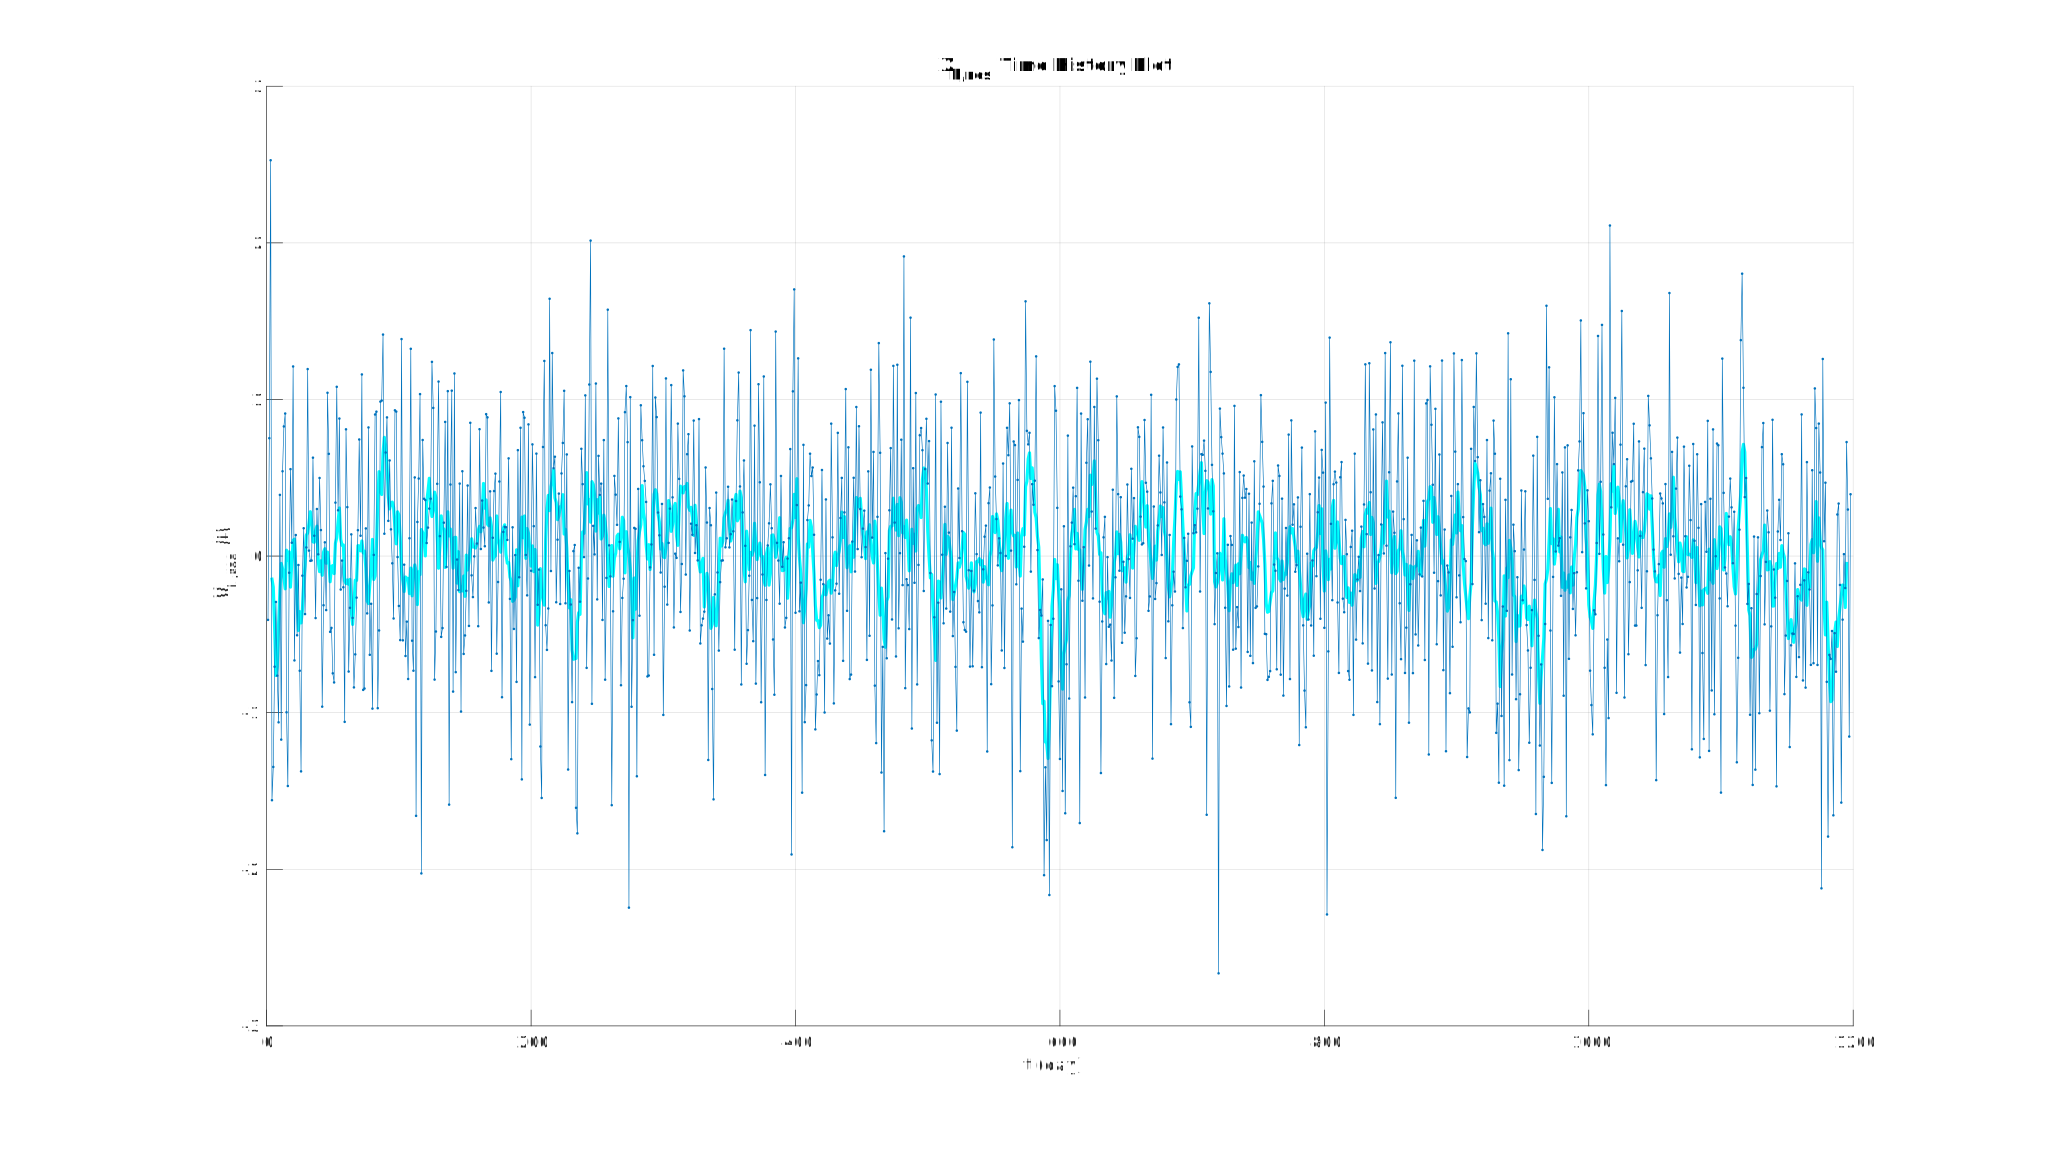
\includegraphics[width=\textwidth]{plots/xb_deseasoned_residuals_history.svg.pdf}
        \caption{Διάγραμμα ιστορίας της χρονοσειράς των υπολοίπων της προσαρμογής του μοντέλου της σχέσης (\ref{eq:xb_deseasoned_model}), $\{X_{b_{deseasoned},res}(t) = \hat{z}(t)\}$}
        \label{fig:xb_deseasoned_residuals_history}
    \end{center}
\end{figure}

Στη συνέχεια δίνονται τα διαγράμματα δειγματικής αυτοσυσχέτισης και \tl{p-values} του \tl{Ljung \& Box test} για μέγιστη υστέρηση $\tau$ από 1 έως 30:

\begin{figure}[H]
    \begin{center}
        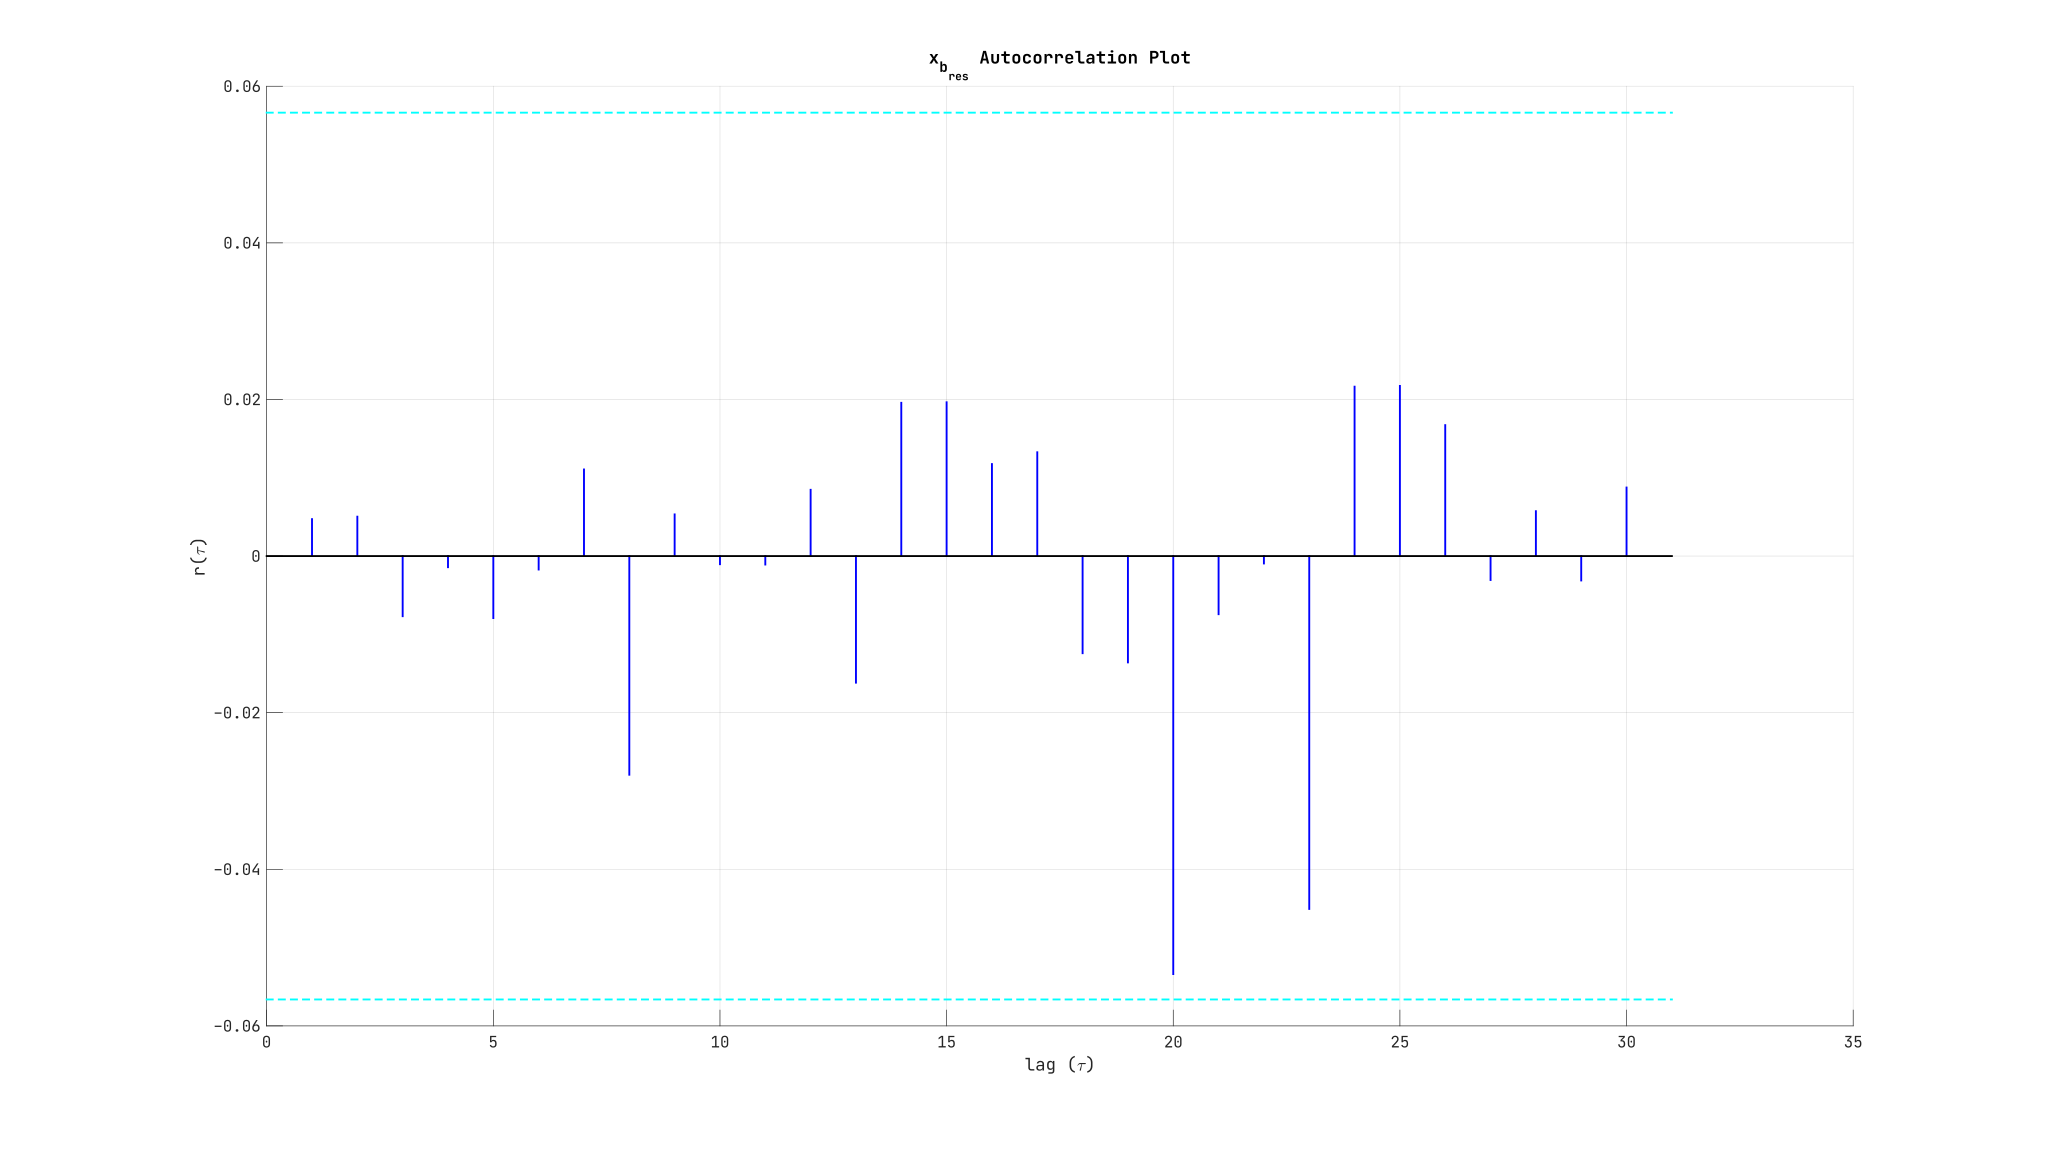
\includegraphics[width=\textwidth]{plots/xb_deseasoned_residuals_autocorrelation.svg.pdf}
        \caption{Διάγραμμα δειγματικής αυτοσυσχέτισης της σειράς των υπολοίπων της προσαρμογής του μοντέλου της σχέσης (\ref{eq:xb_deseasoned_model}), $r_{\hat{z}_b}(\tau)$}
        \label{fig:xb_deseasoned_residuals_autocorrelation}
    \end{center}
\end{figure}

\begin{figure}[H]
    \begin{center}
        \includegraphics[width=\textwidth]{plots/xb_deseasoned_residuals_portmanteau.svg.pdf}
        \caption{Διάγραμμα των \tl{p-values} του στατιστικόυ ελέγχου ανεξαρτησίας \tl{Portmanteau (Ljung \& Box test)} των υπολοίπων της προσαρμογής του μοντέλου της σχέσης (\ref{eq:xb_deseasoned_model}). Σημειώνεται με διακεκομμένη γραμμή το όριο απόφασης όπου όπως φαίνεται η μηδενική υπόθεση $H_0$ (η σειρά των υπολοίπων είναι \tl{iid}) δεν απόρριπτεται για καμία από τις 30 υστερήσεις.}
        \label{fig:xb_deseasoned_residuals_portmanteau}
    \end{center}
\end{figure}

Αμφότερα τα σχήματα \ref{fig:xb_deseasoned_residuals_autocorrelation} και \ref{fig:xb_deseasoned_residuals_portmanteau} παραπάνω φανερώνουν ότι η προσαρμογή του $ARMA(9,9)$ μοντέλου της σχέσης (\ref{eq:xb_deseasoned_model}) είναι επιτυχής αφού αφήνει ασυσχέτιστα υπόλοιπα. Αυτό φαίνεται στο διάγραμμα αυτοσυσχετίσεων των υπολοίπων όπου για καμία υστέρηση η αυτοσυσχέτιση δεν ξεπερνάει το όριο σημαντικότητας, όντας όλες στατιστικά μηδενικές. Αντίστοιχα αποτελέσμστα λαμβάνουμε και από τον έλεγχο ανεξαρτησίας \tl{Portmanteau} όπου η μηδενική υπόθεση πως η σειρά των υπολοίπων είναι \tl{iid} δεν απορρίπτεται για καμία από τις 30 υστερήσεις. Με ασφάλεια μπορούμε να πούμε πως η προσαρμογή αφήνει λευκό θόρυβο ως σειρά υπολοίπων.

\par Τέλος, για λόγους πληρότητας παρεθέτουμε το \tl{NRMSE} των σφαλμάτων προσαρμογής (στη στάσιμη χρονοσειρά) για πρόβλεψη ενός βήματος μπροστά καθώς και τις ίδιες τις προβλέψεις μαζί με την αρχική χρονοσειρά προβολών του βίντεο \tl{B} με βάση τη σχέση (\ref{eq:yb_model}), παρακάτω:

\begin{align}
NRMSE(\hat{X_{b_{deseasoned}}}, X_{b_{deseasoned}}) = 0.7589
\end{align}

\begin{figure}[H]
    \begin{center}
        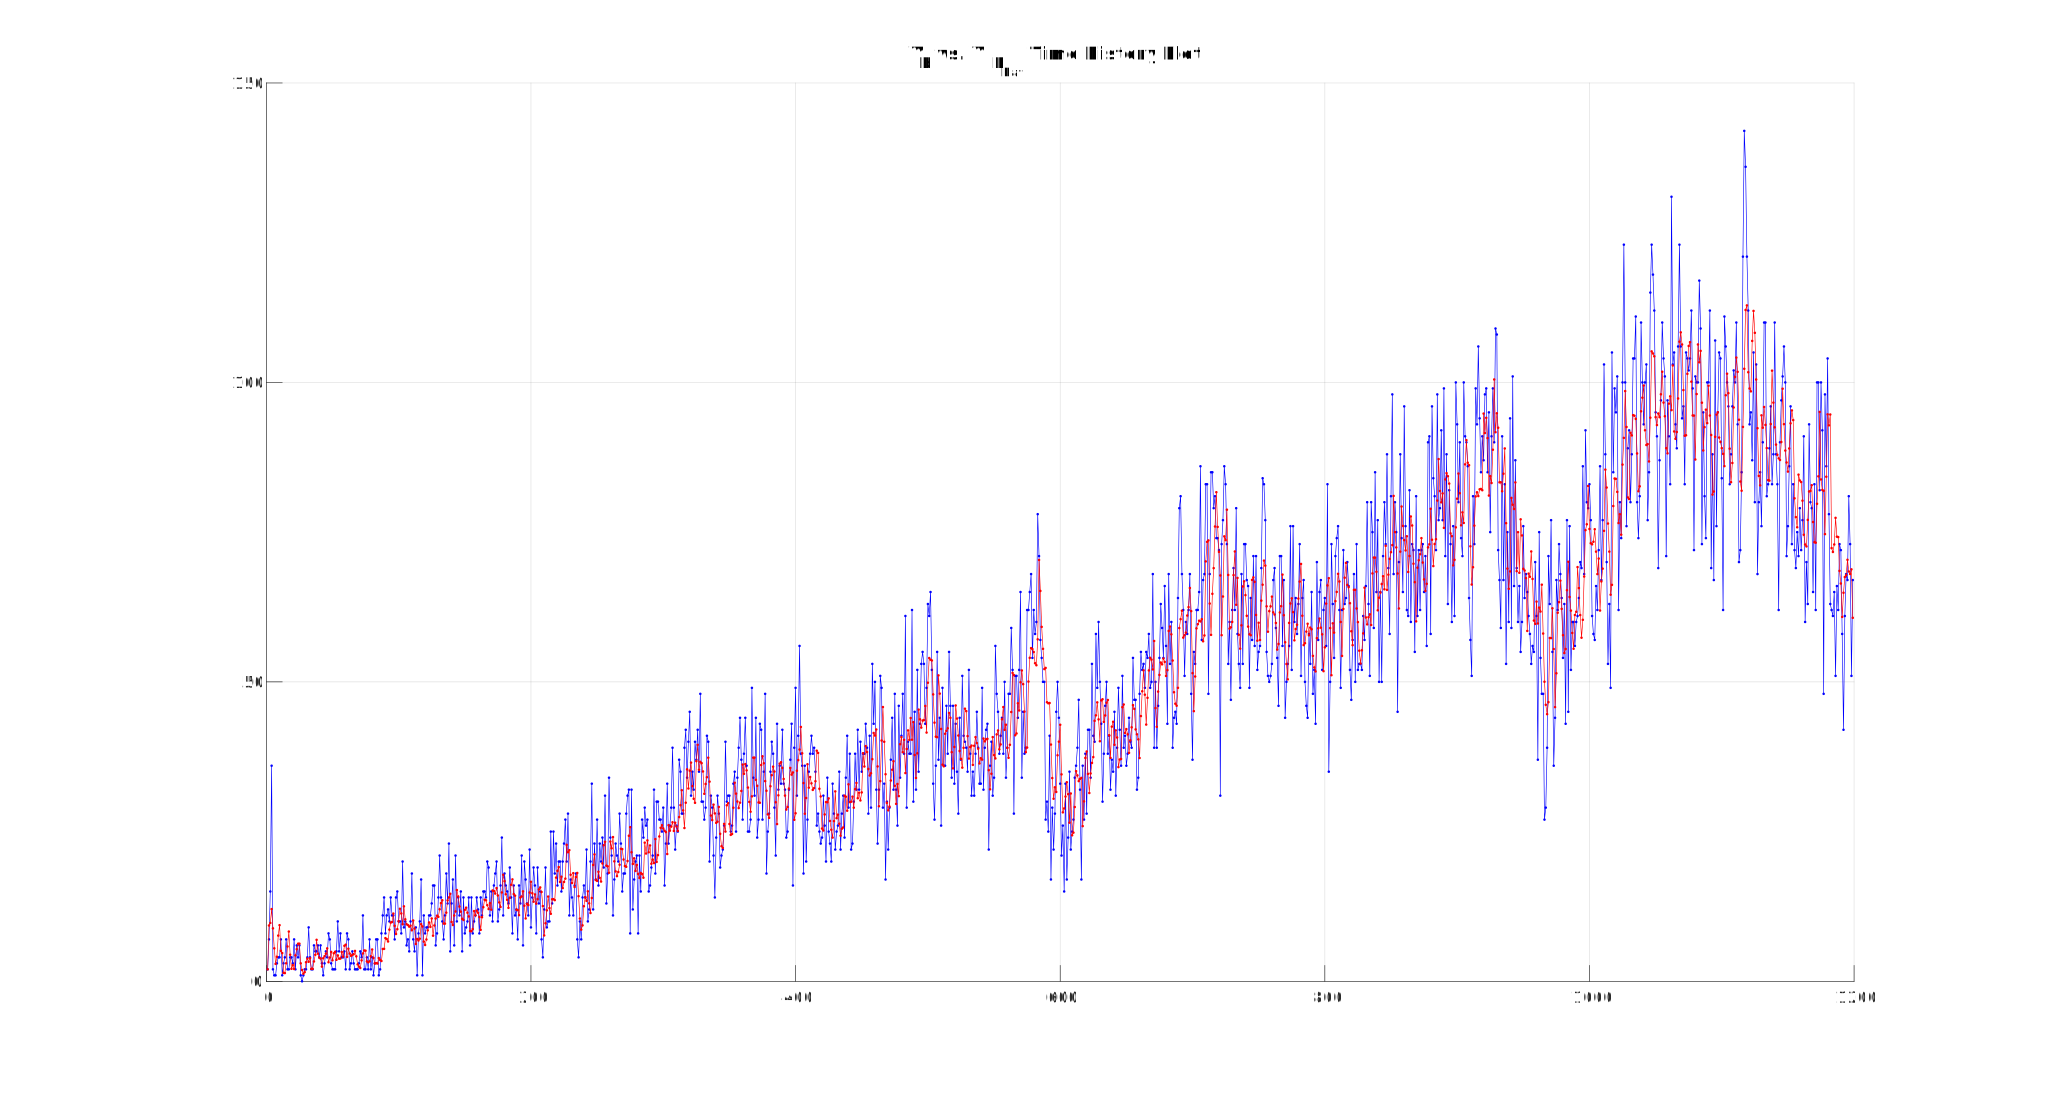
\includegraphics[width=\textwidth]{plots/yb_vs_yb_hat_history.svg.pdf}
        \caption{Διάγραμμα ιστορίας της αρχικής χρονοσειράς προβολών του βίντεο \tl{B} (μπλε) καθώς και τις προβλέψεις ενός βήματος μπροστά αυτής με βάση το προσαρμοσμένο μοντέλο $ARMA(9,9)$ και τη σχέση (\ref{eq:yb_model}) (κόκκινο).}
        \label{fig:yb_vs_yb_hat_history}
    \end{center}
\end{figure}


\section{Διάγνωση καταλληλότητας του μοντέλου \tl{ARMA(4,4)}}

\subsection{Τελικό μοντέλο τύπου \tl{ARMA(4,4)} για τη στάσιμη χρονοσειρά}

Το μοντέλο $ARMA(4,4)$ που εκτιμήθηκε από τη συνάρτηση \texttt{\tl{fitARMA}()} και προσαρμόστηκε στη στάσιμη χρονοσειρά, δηλαδή την απαλλαγμένη από εποχικότητα χρονοσειρά των διαφορών των τετραγωνικών ριζών είναι το εξής:
\begin{flalign}
\begin{aligned}
x_{t_{(4,4)}} = &\ 0.0055 + 0.806x_{t-1_{(4,4)}} - 0.329x_{t-2_{(4,4)}} - 0.570x_{t-3_{(4,4)}} \\
                &+ 0.112x_{t-4_{(4,4)}} + z_t - 1.572z_{t-1} + 0.970z_{t-2} \\
                &+ 0.180z_{t-3} - 0.405z_{t-4}, \ \ \ \ \  t=5,..,1199
\label{eq:xb_deseasoned_4_4_model}
\end{aligned}
\end{flalign}

όπου ο μέσος όρος της στάσιμης χρονοσειράς $\{X_{b_{deseasoned}}(t)\}$ είναι $\overline{x}=0.0055$. Ενώ η εκτίμηση της τυπικής απόκλισης των σφαλμάτων ή υπολοίπων προσαρμογής του $ARMA(4,4)$ βρέθηκε να είναι ίση με \textbf{$s_z = 0.7481$} (εκτίμηση διασποράς ίση με $s_z^2 = 0.5596$), είναι δηλαδή οριακά μεγαλύτερη από τα αντίστοιχα της προσαρμογής $ARMA(9,9)$. Το αντίστοιχο μοντέλο με το οποίο θα προσεγγίζαμε την αρχική χρονοσειρά των προβολών του βίντεο Α, λαμβάνοντας υπόψη και τον εποχικό όρο, θα είναι:
\begin{align}
Y_t = \left(\sqrt{Y_{t-1}} + X_{t_{(4,4)}} + \widetilde{S_b}(t) \right)^2, \ \ \  t=5,..,1199
\label{eq:yb_4_4_model}
\end{align}

\subsection{Διάγνωση Καταλληλότητας \& Σφάλματα Προσαρμογής}

Ακολούθως, θα κάνουμε διάγνωση καταλληλότητας του μοντέλου $ARMA(4,4)$ ακολουθώντας πανομοιότυπη διαδικασία με αυτή της διάγνωσης καταλληλότητας του $ARMA(9,9)$ μοντέλου, δηλαδή κάνοντας έλεγχο ανεξαρτησίας στη σειρά των υπολοίπων τόσο με βάση τη δειγματική τους αυτοσυσχέτιση όσο και με τον έλεγχο \tl{Portmanteau}. Σε πρώτη φάση, όμως, το διάγραμμα ιστορίας της σειράς των υπολοίπων ή σφαλμάτων προσαρμογής δίνεται ακολούθως:

\begin{figure}[H]
    \begin{center}
        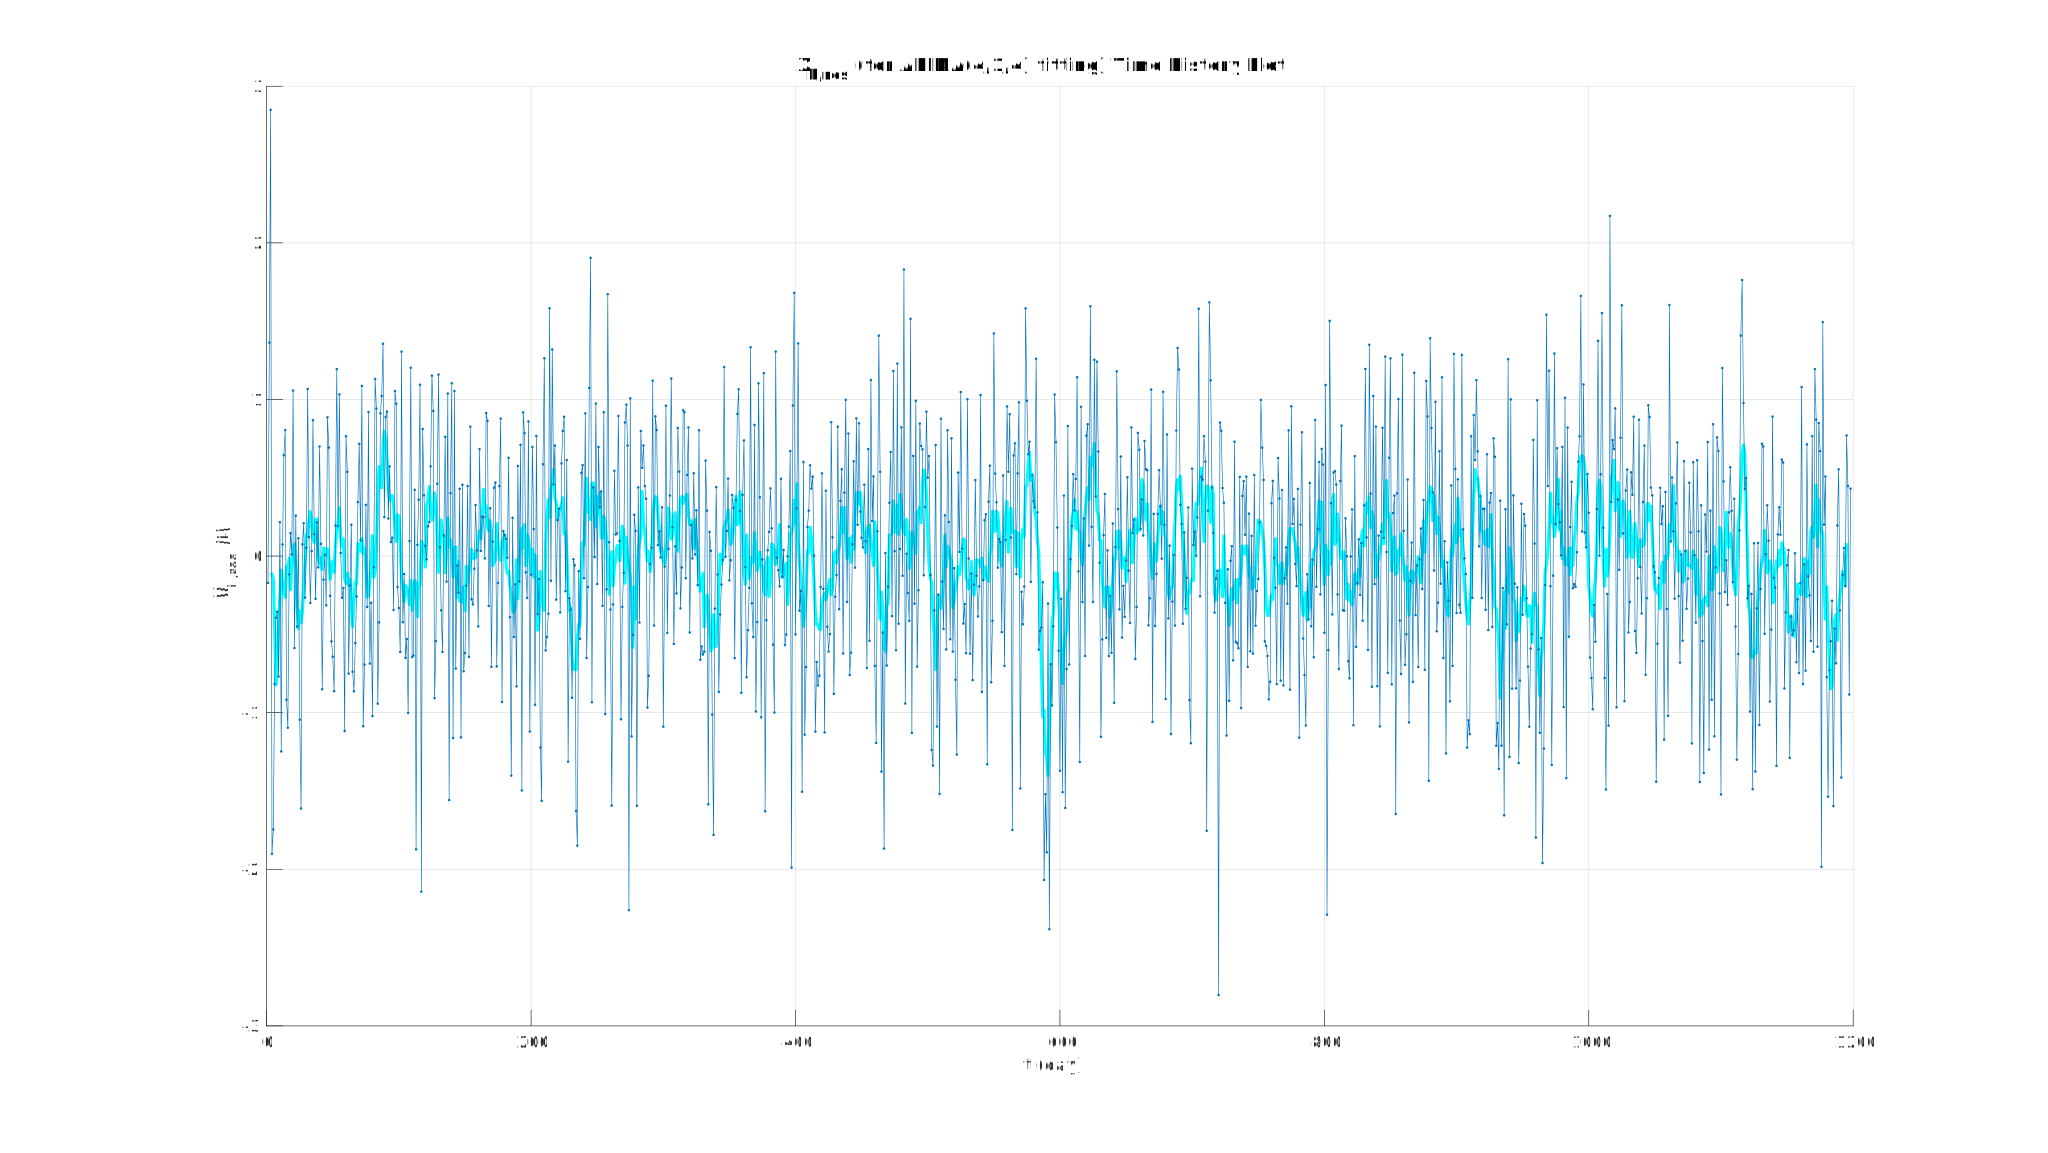
\includegraphics[width=\textwidth]{plots/xb_deseasoned_residuals_4_4_history.svg.pdf}
        \caption{Διάγραμμα ιστορίας της χρονοσειράς των υπολοίπων της προσαρμογής του μοντέλου $ARMA(4,4)$ της σχέσης (\ref{eq:xb_deseasoned_4_4_model}), $\{X_{b_{deseasoned},res(4,4)}(t) = \hat{z}(t)\}$}
        \label{fig:xb_deseasoned_residuals_4_4_history}
    \end{center}
\end{figure}

Στη συνέχεια δίνονται τα διαγράμματα δειγματικής αυτοσυσχέτισης και \tl{p-values} του \tl{Ljung \& Box test} για μέγιστη υστέρηση $\tau$ από 1 έως 30:

\begin{figure}[H]
    \begin{center}
        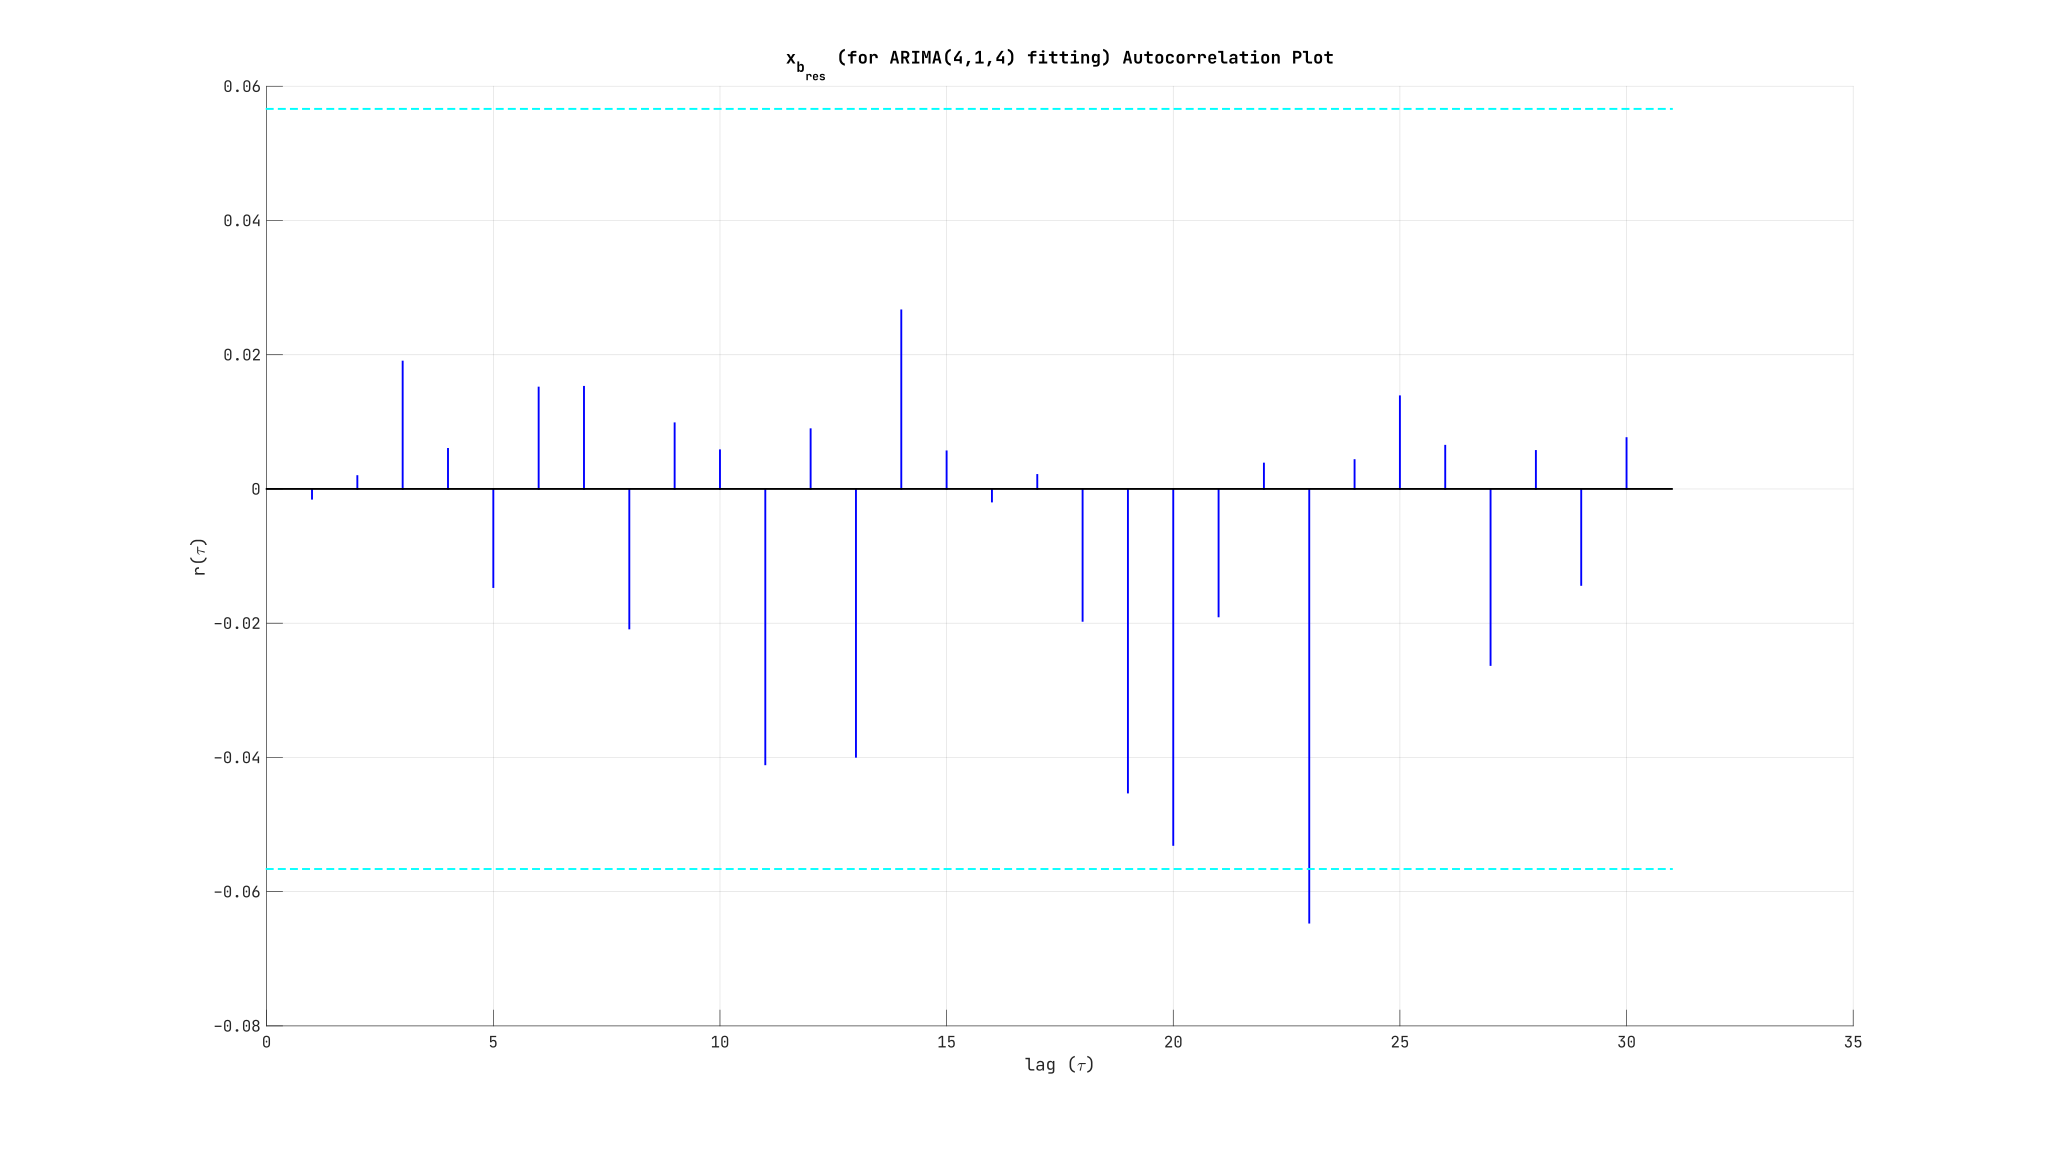
\includegraphics[width=\textwidth]{plots/xb_deseasoned_residuals_4_4_autocorrelation.svg.pdf}
        \caption{Διάγραμμα δειγματικής αυτοσυσχέτισης της σειράς των υπολοίπων της προσαρμογής του μοντέλου $ARMA(4,4)$  της σχέσης (\ref{eq:xb_deseasoned_4_4_model}), $r_{\hat{z}_b}(\tau)$}
        \label{fig:xb_deseasoned_residuals_4_4_autocorrelation}
    \end{center}
\end{figure}

\begin{figure}[H]
    \begin{center}
        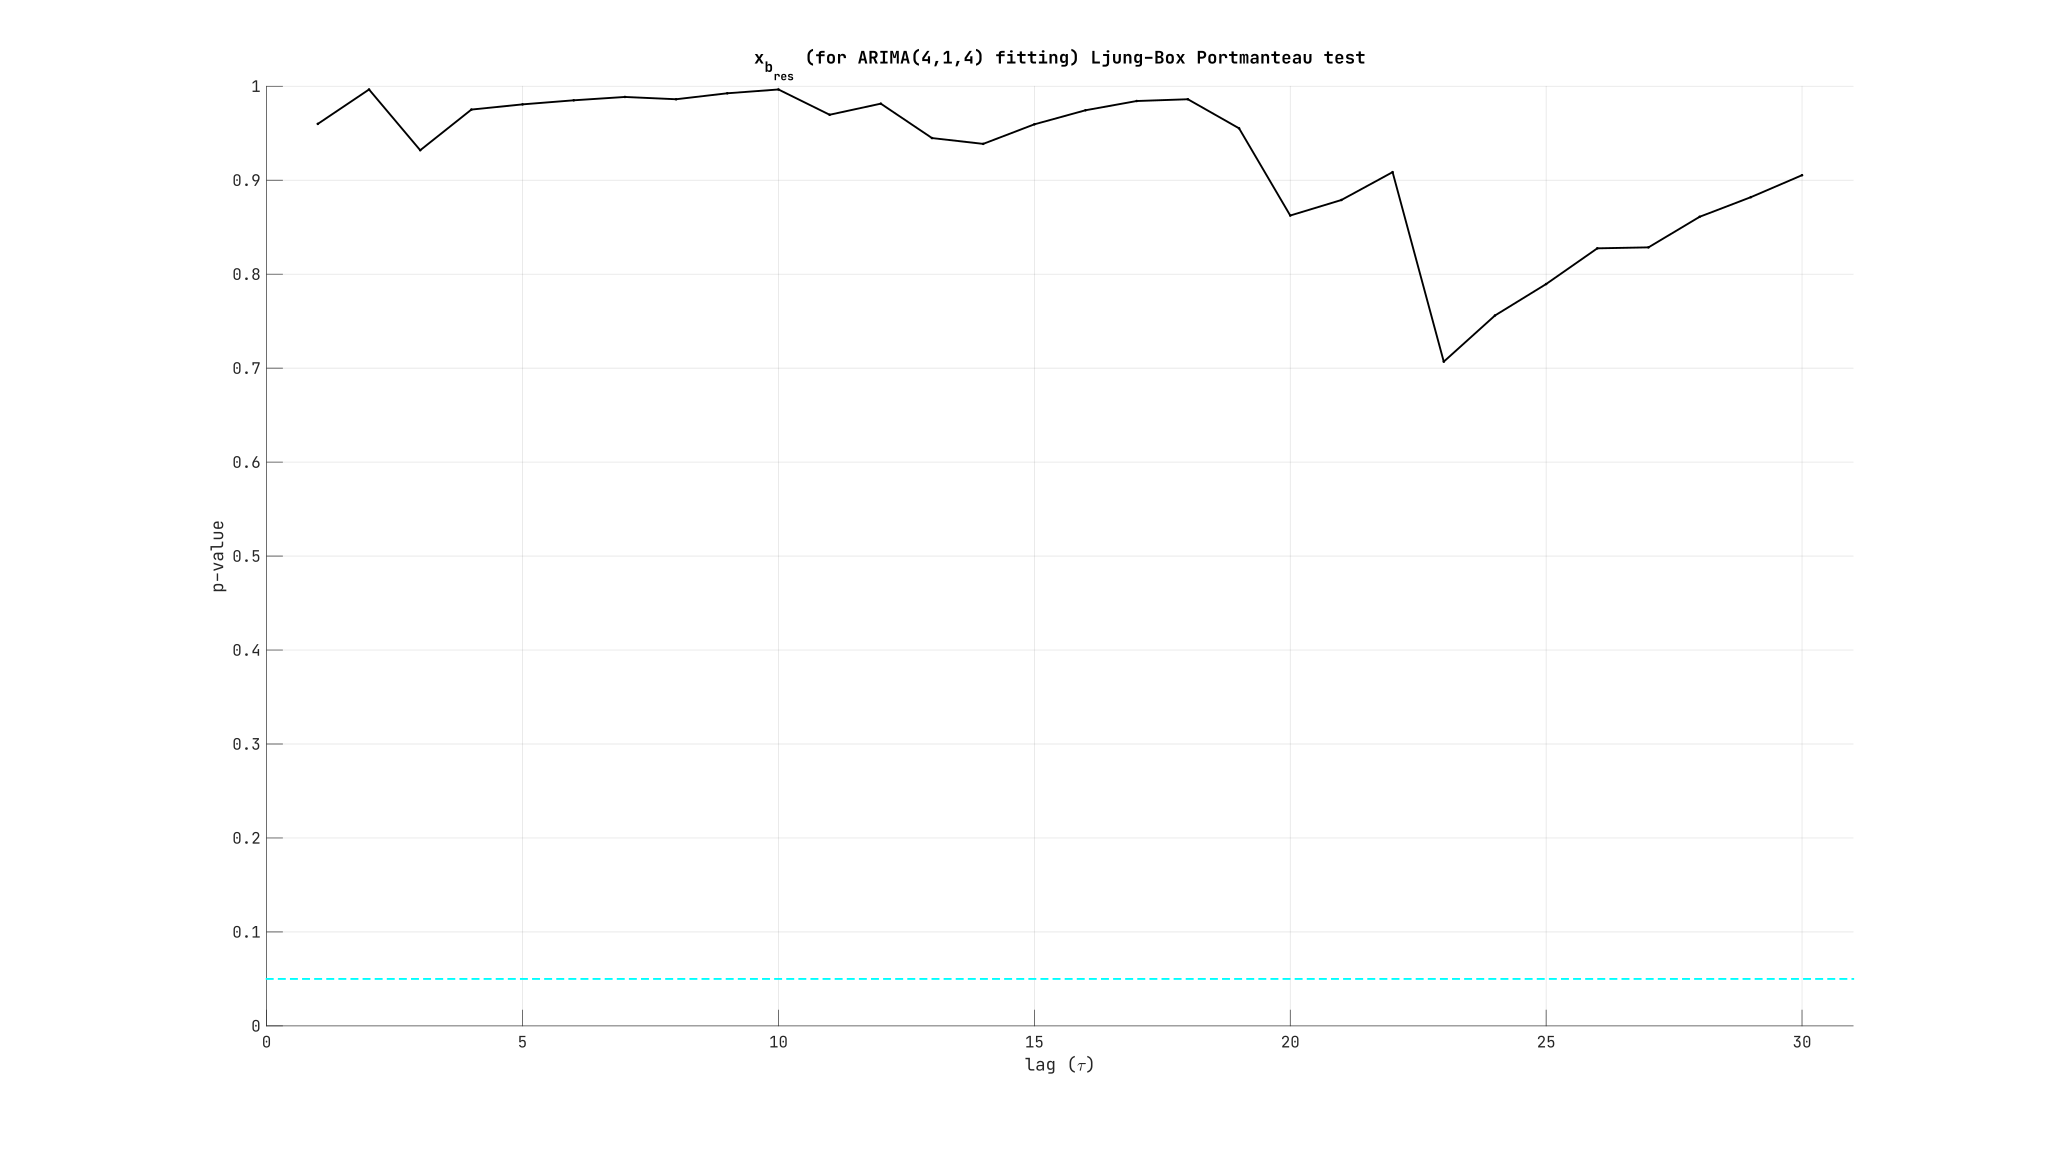
\includegraphics[width=\textwidth]{plots/xb_deseasoned_residuals_4_4_portmanteau.svg.pdf}
        \caption{Διάγραμμα των \tl{p-values} του στατιστικόυ ελέγχου ανεξαρτησίας \tl{Portmanteau (Ljung \& Box test)} των υπολοίπων της προσαρμογής του μοντέλου $ARMA(4,4)$ της σχέσης (\ref{eq:xb_deseasoned_4_4_model}). Σημειώνεται με διακεκομμένη γραμμή το όριο απόφασης όπου όπως φαίνεται η μηδενική υπόθεση $H_0$ (η σειρά των υπολοίπων είναι \tl{iid}) δεν απόρριπτεται για καμία από τις 30 υστερήσεις.}
        \label{fig:xb_deseasoned_residuals_4_4_portmanteau}
    \end{center}
\end{figure}

Αμφότερα τα σχήματα \ref{fig:xb_deseasoned_residuals_4_4_autocorrelation} και \ref{fig:xb_deseasoned_residuals_4_4_portmanteau} παραπάνω φανερώνουν ότι η προσαρμογή του $ARMA(4,4)$ μοντέλου της σχέσης (\ref{eq:xb_deseasoned_4_4_model}) είναι επιτυχής αφού αφήνει ασυσχέτιστα υπόλοιπα. Αυτό φαίνεται στο διάγραμμα αυτοσυσχετίσεων των υπολοίπων όπου μόνο για μία υστέρηση (για $\tau$ 23) η αυτοσυσχέτιση ξεπερνάει το όριο σημαντικότητας (κάτι που επιτρέπεται από το επίπεδο εμπιστοσύνης) ενώ όλες οι υπόλοιπες αυτοσυσχετίσεις είναι στατιστικά μηδενικές. Αντίστοιχα αποτελέσμστα λαμβάνουμε και από τον έλεγχο ανεξαρτησίας \tl{Portmanteau} όπου η μηδενική υπόθεση πως η σειρά των υπολοίπων είναι \tl{iid} δεν απορρίπτεται για καμία από τις 30 υστερήσεις. Με ασφάλεια μπορούμε να πούμε πως η προσαρμογή αφήνει λευκό θόρυβο ως σειρά υπολοίπων.

\par Τέλος, για λόγους πληρότητας παρεθέτουμε το \tl{NRMSE} των σφαλμάτων προσαρμογής του $ARMA(4,4)$ (στη στάσιμη χρονοσειρά) για πρόβλεψη ενός βήματος μπροστά καθώς και τις ίδιες τις προβλέψεις μαζί με την αρχική χρονοσειρά προβολών του βίντεο \tl{B} με βάση τη σχέση (\ref{eq:yb_4_4_model}), παρακάτω:

\begin{align}
NRMSE(\hat{X_{b_{deseasoned,(4,4)}}}, X_{b_{deseasoned}}) = 0.7712
\end{align}

\begin{figure}[H]
    \begin{center}
        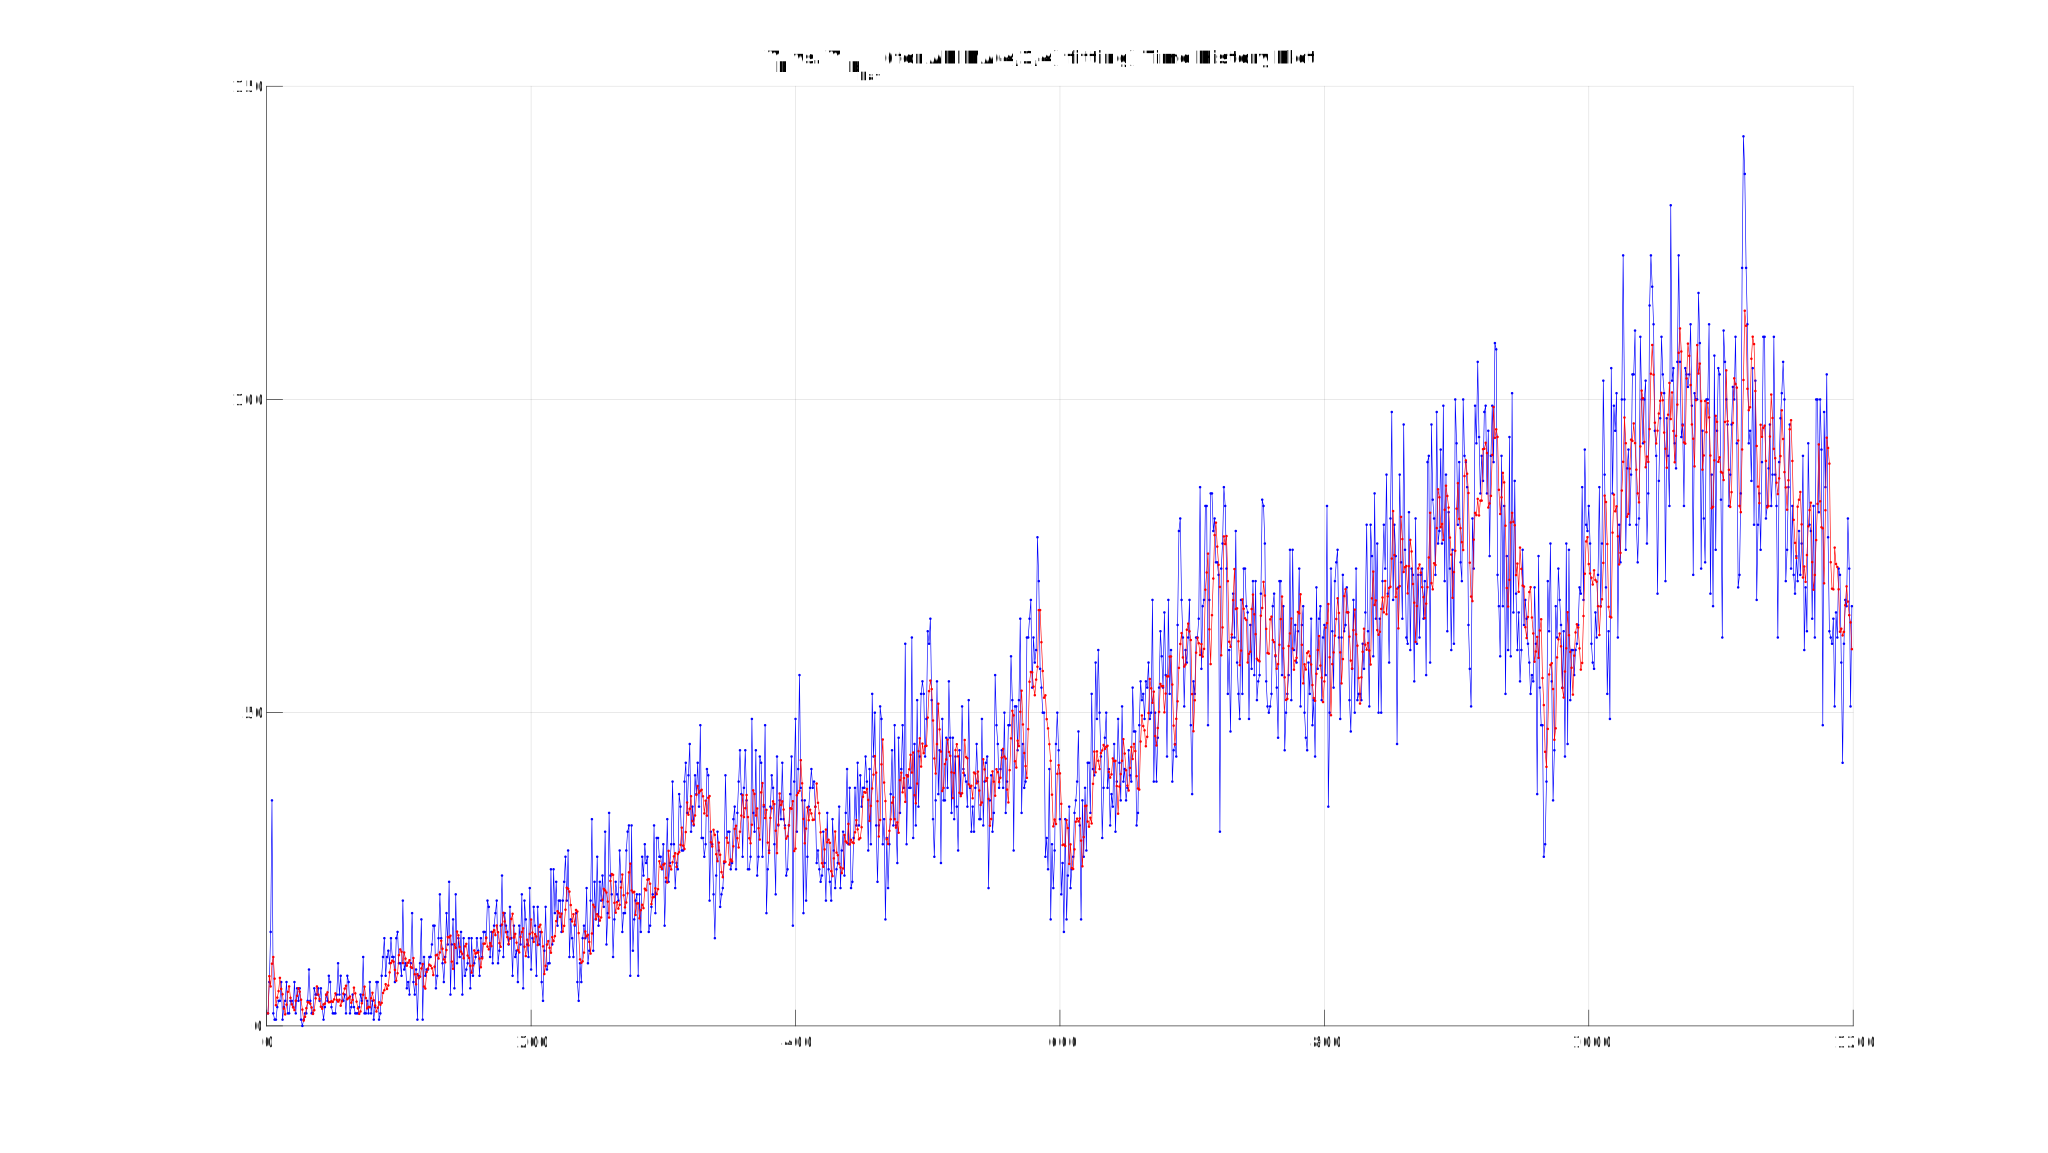
\includegraphics[width=\textwidth]{plots/yb_vs_yb_hat_4_4_history.svg.pdf}
        \caption{Διάγραμμα ιστορίας της αρχικής χρονοσειράς προβολών του βίντεο \tl{B} (μπλε) καθώς και τις προβλέψεις ενός βήματος μπροστά αυτής με βάση το προσαρμοσμένο μοντέλο $ARMA(4,4)$ και τη σχέση (\ref{eq:yb_4_4_model}) (κόκκινο).}
        \label{fig:yb_vs_yb_hat_4_4_history}
    \end{center}
\end{figure}

\subsection{Συμπερασματικά σχόλια}

Βλέποντας λοιπόν από την ανάλυση που προηγήθηκε ότι η προσαρμογή αμφότερων των γραμμικών μοντέλων $ARMA(4,4)$ και $ARMA(9,9)$ οδηγεί σε ασυσχέτιστα υπόλοιπα αντλώντας όλη τη πληροφορία (που μπορεί να αντλήσει ένα γραμμικό μοντέλο) από τη στάστιμη χρονοσειρά, $\{X_{b_{deseasoned}}(t)\}$, καταλήγουμε στο μοντέλο $ARMA(4,4)$ της σχέσης (\ref{eq:xb_deseasoned_4_4_model}) ως το πιο κατάλληλο καθώς το γεγονός ότι έχει μικρότερες τάξεις θα μας οδηγήσει σε πιο ασφαλείς προβλέψεις και μείωση της πιθανότητας \tl{overfitting}.